\documentclass[11pt,a4paper]{article}
\usepackage[margin=24mm]{geometry}

\usepackage[T1]{fontenc}
\usepackage[utf8]{inputenc}
\usepackage{amsmath,amssymb,graphicx,longtable,booktabs,array,calc}
\usepackage{etoolbox,xurl,float,needspace}
\usepackage[numbers,sort&compress]{natbib}
\usepackage[unicode,hidelinks]{hyperref}
\hypersetup{pdfauthor={},pdfsubject={Research manuscript}}
\setcounter{secnumdepth}{0}
\setlength{\emergencystretch}{3em}
\providecommand{\tightlist}{\setlength{\itemsep}{0pt}\setlength{\parskip}{0pt}}
\providecommand{\pandocbounded}[1]{#1}
\makeatletter
\def\maxwidth{\ifdim\Gin@nat@width>\linewidth\linewidth\else\Gin@nat@width\fi}
\def\maxheight{\ifdim\Gin@nat@height>0.72\textheight0.72\textheight\else\Gin@nat@height\fi}
\makeatother
\setkeys{Gin}{width=\maxwidth,height=\maxheight,keepaspectratio}

\renewcommand{\thefigure}{S\arabic{figure}}
\begin{document}
\begin{center}{\Large\bfseries All five seed results and source provenance}\end{center}
\AtBeginEnvironment{longtable}{\small}
Supplementary information for \textbf{Separating First-Step Learning-Rate Faults from Scheduler Delay in Adam Training}.

Journal: SN Computer Science.

Authors: Tivdzua Lubem Noah; Bader Rasheed; Dmitriy S. Vatolin.

Corresponding author: Tivdzua Lubem Noah, Innopolis University, Innopolis, Russia; l.tivdzua@innopolis.university.

Research code, retained records and editable sources: \href{https://github.com/tivdzualubem/warmup-update-budget-acml2026/tree/sncs-submission-2026-11-23}{version sncs-submission-2026-11-23}. \href{https://github.com/tivdzualubem/warmup-update-budget-acml2026/raw/refs/tags/sncs-submission-2026-11-23/submission/sncs-2026-11-23/ESM_2.zip}{Download Online Resource 2: reproducibility package}.

Tables S1-S8 report saved test metrics from validation-selected checkpoints; Tables S9-S12 report paired differences. Scratch values are accuracy; pretrained AG News/DBpedia use macro-F1, WNUT entity F1 and CIFAR accuracy. All entries are percentages. Diagnostic fail-fast/LR-assertion arms have no primary test endpoint and remain n.a. in the 240-job CSV. Original validation-only selection is unchanged.

\Needspace{16\baselineskip}

\section{Table S1 AG News medium-4}\label{table-s1-ag-news-medium-4}

Metric: accuracy.

\begin{longtable}[]{@{}rrrrrr@{}}
\toprule\noalign{}
Seed & Stable & Single bad & Late & Rescue & Corrected \\
\midrule\noalign{}
\endhead
\bottomrule\noalign{}
\endlastfoot
42 & 92.2368 & 50.8816 & 68.8026 & 92.0132 & 92.9079 \\
123 & 92.6447 & 36.9079 & 82.5263 & 92.5395 & 92.7105 \\
456 & 92.4079 & 44.9211 & 63.2895 & 92.4342 & 92.3289 \\
789 & 91.4868 & 50.3553 & 80.6579 & 92.4868 & 92.0658 \\
2026 & 91.9868 & 41.7237 & 71.7368 & 92.4737 & 92.4211 \\
\end{longtable}

\Needspace{16\baselineskip}

\section{Table S2 AG News large-6}\label{table-s2-ag-news-large-6}

Metric: accuracy.

\begin{longtable}[]{@{}rrrrrr@{}}
\toprule\noalign{}
Seed & Stable & Single bad & Late & Rescue & Corrected \\
\midrule\noalign{}
\endhead
\bottomrule\noalign{}
\endlastfoot
42 & 92.6053 & 48.4079 & 69.0789 & 92.4342 & 92.7105 \\
123 & 92.6447 & 35.1447 & 78.6579 & 92.2237 & 92.3158 \\
456 & 92.3816 & 37.0395 & 60.2105 & 92.2500 & 91.8158 \\
789 & 91.7237 & 43.8947 & 61.6053 & 92.2105 & 92.3289 \\
2026 & 92.4868 & 50.5263 & 73.0132 & 92.7500 & 92.4737 \\
\end{longtable}

\Needspace{16\baselineskip}

\section{Table S3 DBpedia medium-4}\label{table-s3-dbpedia-medium-4}

Metric: accuracy.

\begin{longtable}[]{@{}rrrrrr@{}}
\toprule\noalign{}
Seed & Stable & Single bad & Late & Rescue & Corrected \\
\midrule\noalign{}
\endhead
\bottomrule\noalign{}
\endlastfoot
42 & 98.5971 & 37.0914 & 94.6057 & 98.5957 & 98.6543 \\
123 & 98.6214 & 27.8714 & 93.8214 & 98.6700 & 98.6829 \\
456 & 98.6257 & 26.0743 & 92.4586 & 98.6471 & 98.6743 \\
789 & 98.6371 & 30.8171 & 92.6243 & 98.6414 & 98.6214 \\
2026 & 98.5971 & 43.5786 & 91.0986 & 98.6357 & 98.7157 \\
\end{longtable}

\Needspace{16\baselineskip}

\section{Table S4 DBpedia large-6}\label{table-s4-dbpedia-large-6}

Metric: accuracy.

\begin{longtable}[]{@{}rrrrrr@{}}
\toprule\noalign{}
Seed & Stable & Single bad & Late & Rescue & Corrected \\
\midrule\noalign{}
\endhead
\bottomrule\noalign{}
\endlastfoot
42 & 98.7943 & 26.7257 & 87.9757 & 98.6714 & 98.6500 \\
123 & 98.7500 & 26.4714 & 61.8986 & 98.6700 & 98.4586 \\
456 & 98.8314 & 24.8686 & 86.1586 & 98.5857 & 98.5629 \\
789 & 98.7529 & 32.0700 & 83.8486 & 98.6686 & 98.5186 \\
2026 & 98.8314 & 28.8814 & 90.7957 & 98.6043 & 98.7071 \\
\end{longtable}

\Needspace{16\baselineskip}

\section{Table S5 AG News distilbert}\label{table-s5-ag-news-distilbert}

Metric: macro-F1.

\begin{longtable}[]{@{}rrrrr@{}}
\toprule\noalign{}
Seed & Safe & Single bad & Late & Rescue \\
\midrule\noalign{}
\endhead
\bottomrule\noalign{}
\endlastfoot
42 & 94.3634 & 94.3483 & 94.4156 & 94.4007 \\
123 & 94.2930 & 94.2683 & 94.2816 & 94.3068 \\
456 & 94.5304 & 94.5050 & 94.4923 & 94.4515 \\
789 & 94.3067 & 94.3208 & 94.3334 & 94.3058 \\
2026 & 94.4129 & 94.4671 & 94.3752 & 94.5189 \\
\end{longtable}

\Needspace{16\baselineskip}

\section{Table S6 DBpedia distilbert}\label{table-s6-dbpedia-distilbert}

Metric: macro-F1.

\begin{longtable}[]{@{}rrrrr@{}}
\toprule\noalign{}
Seed & Safe & Single bad & Late & Rescue \\
\midrule\noalign{}
\endhead
\bottomrule\noalign{}
\endlastfoot
42 & 99.2814 & 99.2958 & 99.2886 & 99.3000 \\
123 & 99.3056 & 99.2999 & 99.2870 & 99.2970 \\
456 & 99.3100 & 99.3043 & 99.3000 & 99.3115 \\
789 & 99.2857 & 99.2943 & 99.2799 & 99.2758 \\
2026 & 99.2899 & 99.2971 & 99.3086 & 99.2713 \\
\end{longtable}

\Needspace{16\baselineskip}

\section{Table S7 WNUT-17 distilbert}\label{table-s7-wnut-17-distilbert}

Metric: entity F1.

\begin{longtable}[]{@{}rrrrr@{}}
\toprule\noalign{}
Seed & Safe & Single bad & Late & Rescue \\
\midrule\noalign{}
\endhead
\bottomrule\noalign{}
\endlastfoot
42 & 43.2463 & 43.5912 & 43.4635 & 43.4635 \\
123 & 42.4561 & 42.2650 & 42.3077 & 42.3077 \\
456 & 39.6135 & 40.2644 & 39.9036 & 39.9036 \\
789 & 43.5227 & 43.3638 & 43.2895 & 43.2895 \\
2026 & 42.5532 & 42.9630 & 42.5873 & 42.5873 \\
\end{longtable}

\Needspace{16\baselineskip}

\section{Table S8 CIFAR-10 deit-tiny}\label{table-s8-cifar-10-deit-tiny}

Metric: accuracy.

\begin{longtable}[]{@{}rrrrr@{}}
\toprule\noalign{}
Seed & Safe & Single bad & Late & Rescue \\
\midrule\noalign{}
\endhead
\bottomrule\noalign{}
\endlastfoot
42 & 96.2900 & 96.3000 & 96.2000 & 96.4100 \\
123 & 96.3000 & 96.1000 & 96.2600 & 95.9700 \\
456 & 95.9900 & 96.0500 & 96.0900 & 96.0600 \\
789 & 96.0900 & 96.1700 & 96.1700 & 96.0600 \\
2026 & 96.2700 & 96.2200 & 95.8300 & 96.2800 \\
\end{longtable}

\Needspace{16\baselineskip}

\section{Table S9 Paired differences AG News medium-4}\label{table-s9-paired-differences-ag-news-medium-4}

All differences are percentage points. The repair and remaining-delay columns are exploratory.

\begin{longtable}[]{@{}rrrr@{}}
\toprule\noalign{}
Seed & Stable - bad & Rescue - late & Corrected - rescue \\
\midrule\noalign{}
\endhead
\bottomrule\noalign{}
\endlastfoot
42 & +41.35526 & +23.21053 & +0.89474 \\
123 & +55.73684 & +10.01316 & +0.17105 \\
456 & +47.48684 & +29.14474 & -0.10526 \\
789 & +41.13158 & +11.82895 & -0.42105 \\
2026 & +50.26316 & +20.73684 & -0.05263 \\
\end{longtable}

\Needspace{16\baselineskip}

\section{Table S10 Paired differences AG News large-6}\label{table-s10-paired-differences-ag-news-large-6}

All differences are percentage points. The repair and remaining-delay columns are exploratory.

\begin{longtable}[]{@{}rrrr@{}}
\toprule\noalign{}
Seed & Stable - bad & Rescue - late & Corrected - rescue \\
\midrule\noalign{}
\endhead
\bottomrule\noalign{}
\endlastfoot
42 & +44.19737 & +23.35526 & +0.27632 \\
123 & +57.50000 & +13.56579 & +0.09211 \\
456 & +55.34211 & +32.03947 & -0.43421 \\
789 & +47.82895 & +30.60526 & +0.11842 \\
2026 & +41.96053 & +19.73684 & -0.27632 \\
\end{longtable}

\Needspace{16\baselineskip}

\section{Table S11 Paired differences DBpedia medium-4}\label{table-s11-paired-differences-dbpedia-medium-4}

All differences are percentage points. The repair and remaining-delay columns are exploratory.

\begin{longtable}[]{@{}rrrr@{}}
\toprule\noalign{}
Seed & Stable - bad & Rescue - late & Corrected - rescue \\
\midrule\noalign{}
\endhead
\bottomrule\noalign{}
\endlastfoot
42 & +61.50571 & +3.99000 & +0.05857 \\
123 & +70.75000 & +4.84857 & +0.01286 \\
456 & +72.55143 & +6.18857 & +0.02714 \\
789 & +67.82000 & +6.01714 & -0.02000 \\
2026 & +55.01857 & +7.53714 & +0.08000 \\
\end{longtable}

\Needspace{16\baselineskip}

\section{Table S12 Paired differences DBpedia large-6}\label{table-s12-paired-differences-dbpedia-large-6}

All differences are percentage points. The repair and remaining-delay columns are exploratory.

\begin{longtable}[]{@{}rrrr@{}}
\toprule\noalign{}
Seed & Stable - bad & Rescue - late & Corrected - rescue \\
\midrule\noalign{}
\endhead
\bottomrule\noalign{}
\endlastfoot
42 & +72.06857 & +10.69571 & -0.02143 \\
123 & +72.27857 & +36.77143 & -0.21143 \\
456 & +73.96286 & +12.42714 & -0.02286 \\
789 & +66.68286 & +14.82000 & -0.15000 \\
2026 & +69.95000 & +7.80857 & +0.10286 \\
\end{longtable}

\section{Selection and provenance}\label{selection-and-provenance}

Source manifest: tables/manuscript\_table\_sources.json. The \path{all_condition_results.csv} file records the exact result member, selection metric and selected epoch for every job. The \path{paired_per_seed.csv} file records both source members and realized optimizer budgets. Pretrained selection is also exported in \path{pretrained_selection_and_primary_metric.csv}. Selection scores and epochs agree with the saved histories. Historical checkpoint weights are absent from the October archive; new-pair states are reported separately below.

The five-seed paired summaries use sample SD and descriptive 95\% Student-t intervals. A two-sided exact sign test has p=0.0625 for five same-direction differences; this does not meet an unadjusted 0.05 threshold. No equivalence margin was prespecified. The historical three-seed sweep is a distinct protocol.

\Needspace{16\baselineskip}

\section{Table S13 Archived scratch training and selected test performance}\label{table-s13-archived-scratch-training-and-selected-test-performance}

Loss values retain the archived mean-of-batch-means logit CE definition. Entries are five-seed means evaluated with the minimum-validation-loss checkpoint. Diagnostic fail-fast arms have no trained-model endpoint (n.a.). These checkpoint evaluations differ from online training loss recorded while dropout and changing weights are active.

\begin{longtable}[]{@{}
  >{\raggedright\arraybackslash}p{(\linewidth - 8\tabcolsep) * \real{0.2000}}
  >{\raggedright\arraybackslash}p{(\linewidth - 8\tabcolsep) * \real{0.2000}}
  >{\raggedleft\arraybackslash}p{(\linewidth - 8\tabcolsep) * \real{0.2000}}
  >{\raggedleft\arraybackslash}p{(\linewidth - 8\tabcolsep) * \real{0.2000}}
  >{\raggedleft\arraybackslash}p{(\linewidth - 8\tabcolsep) * \real{0.2000}}@{}}
\toprule\noalign{}
\begin{minipage}[b]{\linewidth}\raggedright
Setting
\end{minipage} & \begin{minipage}[b]{\linewidth}\raggedright
Condition
\end{minipage} & \begin{minipage}[b]{\linewidth}\raggedleft
Archived train loss
\end{minipage} & \begin{minipage}[b]{\linewidth}\raggedleft
Train accuracy (\%)
\end{minipage} & \begin{minipage}[b]{\linewidth}\raggedleft
Test accuracy (\%)
\end{minipage} \\
\midrule\noalign{}
\endhead
\bottomrule\noalign{}
\endlastfoot
AG News medium-4 & Stable & 0.141 & 95.24 & 92.15 \\
AG News medium-4 & Bad then stable & 207.923 & 45.75 & 44.96 \\
AG News medium-4 & Correct legacy & 0.129 & 95.71 & 92.49 \\
AG News medium-4 & Late legacy & 6.100 & 75.26 & 73.40 \\
AG News medium-4 & Rescue & 0.140 & 95.32 & 92.39 \\
AG News medium-4 & Fail-fast & n.a. & n.a. & n.a. \\
AG News large-6 & Stable & 0.119 & 95.96 & 92.37 \\
AG News large-6 & Bad then stable & 1,207.031 & 43.26 & 43.00 \\
AG News large-6 & Correct legacy & 0.132 & 95.67 & 92.33 \\
AG News large-6 & Late legacy & 198.833 & 70.57 & 68.51 \\
AG News large-6 & Rescue & 0.137 & 95.53 & 92.37 \\
AG News large-6 & Fail-fast & n.a. & n.a. & n.a. \\
DBpedia medium-4 & Stable & 0.040 & 99.01 & 98.62 \\
DBpedia medium-4 & Bad then stable & 424.333 & 33.07 & 33.09 \\
DBpedia medium-4 & Correct legacy & 0.033 & 99.13 & 98.67 \\
DBpedia medium-4 & Late legacy & 0.761 & 93.38 & 92.92 \\
DBpedia medium-4 & Rescue & 0.031 & 99.18 & 98.64 \\
DBpedia medium-4 & Fail-fast & n.a. & n.a. & n.a. \\
DBpedia large-6 & Stable & 0.023 & 99.44 & 98.79 \\
DBpedia large-6 & Bad then stable & 2,338.591 & 27.80 & 27.80 \\
DBpedia large-6 & Correct legacy & 0.037 & 99.11 & 98.58 \\
DBpedia large-6 & Late legacy & 119.595 & 82.56 & 82.14 \\
DBpedia large-6 & Rescue & 0.034 & 99.22 & 98.64 \\
DBpedia large-6 & Fail-fast & n.a. & n.a. & n.a. \\
\end{longtable}

\Needspace{16\baselineskip}

\section{Table S14 Scratch positive-LR, zero-LR and replay budgets}\label{table-s14-scratch-positive-lr-zero-lr-and-replay-budgets}

Each row is a separate five-job mean. Positive-LR and zero-LR counts refer to committed transitions; extra replay calls are rejected-candidate overhead, not additional retained training steps. Early stopping makes observed budgets unequal across conditions.

\begin{longtable}[]{@{}
  >{\raggedright\arraybackslash}p{(\linewidth - 8\tabcolsep) * \real{0.2000}}
  >{\raggedright\arraybackslash}p{(\linewidth - 8\tabcolsep) * \real{0.2000}}
  >{\raggedleft\arraybackslash}p{(\linewidth - 8\tabcolsep) * \real{0.2000}}
  >{\raggedleft\arraybackslash}p{(\linewidth - 8\tabcolsep) * \real{0.2000}}
  >{\raggedleft\arraybackslash}p{(\linewidth - 8\tabcolsep) * \real{0.2000}}@{}}
\toprule\noalign{}
\begin{minipage}[b]{\linewidth}\raggedright
Setting
\end{minipage} & \begin{minipage}[b]{\linewidth}\raggedright
Condition
\end{minipage} & \begin{minipage}[b]{\linewidth}\raggedleft
Positive-LR steps
\end{minipage} & \begin{minipage}[b]{\linewidth}\raggedleft
Zero-LR steps
\end{minipage} & \begin{minipage}[b]{\linewidth}\raggedleft
Extra replay calls
\end{minipage} \\
\midrule\noalign{}
\endhead
\bottomrule\noalign{}
\endlastfoot
AG News medium-4 & Stable & 33,793 & 0 & 0.0 \\
AG News medium-4 & Bad then stable & 49,999 & 8,023 & 0.0 \\
AG News medium-4 & Correct legacy & 26,779 & 0 & 0.0 \\
AG News medium-4 & Late legacy & 87,351 & 0 & 0.0 \\
AG News medium-4 & Rescue & 25,504 & 0 & 1.0 \\
AG News medium-4 & Fail-fast & 1 & 0 & 0.0 \\
AG News large-6 & Stable & 29,330 & 0 & 0.0 \\
AG News large-6 & Bad then stable & 47,013 & 7,821 & 0.0 \\
AG News large-6 & Correct legacy & 26,779 & 0 & 0.0 \\
AG News large-6 & Late legacy & 87,989 & 0 & 0.0 \\
AG News large-6 & Rescue & 26,142 & 0 & 1.0 \\
AG News large-6 & Fail-fast & 1 & 0 & 0.0 \\
DBpedia medium-4 & Stable & 49,999 & 80,901 & 0.0 \\
DBpedia medium-4 & Bad then stable & 49,999 & 80,901 & 0.0 \\
DBpedia medium-4 & Correct legacy & 124,950 & 0 & 0.0 \\
DBpedia medium-4 & Late legacy & 446,250 & 0 & 0.0 \\
DBpedia medium-4 & Rescue & 133,875 & 0 & 1.0 \\
DBpedia medium-4 & Fail-fast & 1 & 0 & 0.0 \\
DBpedia large-6 & Stable & 49,999 & 77,926 & 0.0 \\
DBpedia large-6 & Bad then stable & 49,999 & 69,001 & 0.0 \\
DBpedia large-6 & Correct legacy & 121,975 & 0 & 0.0 \\
DBpedia large-6 & Late legacy & 324,275 & 0 & 0.0 \\
DBpedia large-6 & Rescue & 130,900 & 0 & 1.0 \\
DBpedia large-6 & Fail-fast & 1 & 0 & 0.0 \\
\end{longtable}

\Needspace{16\baselineskip}

\section{Table S15 Pretrained training performance and budgets}\label{table-s15-pretrained-training-performance-and-budgets}

Entries are separate five-job means. The logs preserve online training CE, not a final train-set accuracy evaluation. n.a. denotes an arm that stopped before any complete logged epoch. Safe and single-bad-then-correct schedules reach zero on their final transition; late/rescue schedules can consume the previous positive LR at that transition. A WNUT fail-fast arm can finish training when its guard does not trigger, while remaining a diagnostic condition without a primary test endpoint.

\begin{longtable}[]{@{}
  >{\raggedright\arraybackslash}p{(\linewidth - 8\tabcolsep) * \real{0.2000}}
  >{\raggedright\arraybackslash}p{(\linewidth - 8\tabcolsep) * \real{0.2000}}
  >{\raggedleft\arraybackslash}p{(\linewidth - 8\tabcolsep) * \real{0.2000}}
  >{\raggedleft\arraybackslash}p{(\linewidth - 8\tabcolsep) * \real{0.2000}}
  >{\raggedleft\arraybackslash}p{(\linewidth - 8\tabcolsep) * \real{0.2000}}@{}}
\toprule\noalign{}
\begin{minipage}[b]{\linewidth}\raggedright
Task
\end{minipage} & \begin{minipage}[b]{\linewidth}\raggedright
Condition
\end{minipage} & \begin{minipage}[b]{\linewidth}\raggedleft
Archived online train loss
\end{minipage} & \begin{minipage}[b]{\linewidth}\raggedleft
Positive-LR steps
\end{minipage} & \begin{minipage}[b]{\linewidth}\raggedleft
Zero-LR steps
\end{minipage} \\
\midrule\noalign{}
\endhead
\bottomrule\noalign{}
\endlastfoot
AG News & Safe & 0.099 & 9,563 & 1 \\
AG News & Late & 0.099 & 9,564 & 0 \\
AG News & Single bad & 0.099 & 9,563 & 1 \\
AG News & Rescue & 0.099 & 9,564 & 0 \\
AG News & Fail-fast & n.a. & 1 & 0 \\
AG News & LR assertion & n.a. & 0 & 0 \\
DBpedia & Safe & 0.013 & 44,624 & 1 \\
DBpedia & Late & 0.013 & 44,625 & 0 \\
DBpedia & Single bad & 0.013 & 44,624 & 1 \\
DBpedia & Rescue & 0.013 & 44,625 & 0 \\
DBpedia & Fail-fast & n.a. & 1 & 0 \\
DBpedia & LR assertion & n.a. & 0 & 0 \\
WNUT-17 & Safe & 0.083 & 638 & 1 \\
WNUT-17 & Late & 0.082 & 639 & 0 \\
WNUT-17 & Single bad & 0.082 & 638 & 1 \\
WNUT-17 & Rescue & 0.082 & 639 & 0 \\
WNUT-17 & Fail-fast & 0.082 & 639 & 0 \\
WNUT-17 & LR assertion & n.a. & 0 & 0 \\
CIFAR-10 & Safe & 0.035 & 4,220 & 1 \\
CIFAR-10 & Late & 0.035 & 4,221 & 0 \\
CIFAR-10 & Single bad & 0.035 & 4,220 & 1 \\
CIFAR-10 & Rescue & 0.035 & 4,221 & 0 \\
CIFAR-10 & Fail-fast & n.a. & 1 & 0 \\
CIFAR-10 & LR assertion & n.a. & 0 & 0 \\
\end{longtable}

\Needspace{16\baselineskip}

\section{Table S16 Historical initial-rate severity study}\label{table-s16-historical-initial-rate-severity-study}

Values are test accuracy in percent, mean plus/minus recomputed sample SD across three seeds (42, 123, 456), with 4,000 warmup steps. Rates were consumed as initial rates under the legacy buggy-order protocol.

\begin{longtable}[]{@{}
  >{\raggedright\arraybackslash}p{(\linewidth - 10\tabcolsep) * \real{0.1667}}
  >{\raggedleft\arraybackslash}p{(\linewidth - 10\tabcolsep) * \real{0.1667}}
  >{\raggedleft\arraybackslash}p{(\linewidth - 10\tabcolsep) * \real{0.1667}}
  >{\raggedleft\arraybackslash}p{(\linewidth - 10\tabcolsep) * \real{0.1667}}
  >{\raggedleft\arraybackslash}p{(\linewidth - 10\tabcolsep) * \real{0.1667}}
  >{\raggedleft\arraybackslash}p{(\linewidth - 10\tabcolsep) * \real{0.1667}}@{}}
\toprule\noalign{}
\begin{minipage}[b]{\linewidth}\raggedright
Dataset / architecture
\end{minipage} & \begin{minipage}[b]{\linewidth}\raggedleft
LR 1.0
\end{minipage} & \begin{minipage}[b]{\linewidth}\raggedleft
LR 0.30
\end{minipage} & \begin{minipage}[b]{\linewidth}\raggedleft
LR 0.10
\end{minipage} & \begin{minipage}[b]{\linewidth}\raggedleft
LR 0.03
\end{minipage} & \begin{minipage}[b]{\linewidth}\raggedleft
LR 0.01
\end{minipage} \\
\midrule\noalign{}
\endhead
\bottomrule\noalign{}
\endlastfoot
AG News / medium-4 & 72.02 \(\pm\) 11.94 & 90.43 \(\pm\) 0.64 & 92.44 \(\pm\) 0.05 & 92.56 \(\pm\) 0.11 & 92.69 \(\pm\) 0.20 \\
AG News / large-6 & 78.47 \(\pm\) 1.54 & 86.48 \(\pm\) 1.35 & 91.71 \(\pm\) 0.47 & 92.64 \(\pm\) 0.07 & 92.16 \(\pm\) 0.58 \\
DBpedia / medium-4 & 89.60 \(\pm\) 3.21 & 98.50 \(\pm\) 0.06 & 98.68 \(\pm\) 0.05 & 98.63 \(\pm\) 0.03 & 98.61 \(\pm\) 0.04 \\
DBpedia / large-6 & 82.80 \(\pm\) 8.85 & 97.02 \(\pm\) 0.19 & 98.43 \(\pm\) 0.08 & 98.62 \(\pm\) 0.08 & 98.59 \(\pm\) 0.04 \\
\end{longtable}

\Needspace{16\baselineskip}

\section{Table S17 Retrospective threshold sensitivity}\label{table-s17-retrospective-threshold-sensitivity}

The primary multiplier is 10; every other row is retrospective. Held-out safe counts are transition counts, not independent Bernoulli trials or prospective false-positive certificates. Each threshold excludes the held-out seed and uses only safe steps 1-100.

\begin{longtable}[]{@{}
  >{\raggedleft\arraybackslash}p{(\linewidth - 8\tabcolsep) * \real{0.2000}}
  >{\raggedleft\arraybackslash}p{(\linewidth - 8\tabcolsep) * \real{0.2000}}
  >{\raggedleft\arraybackslash}p{(\linewidth - 8\tabcolsep) * \real{0.2000}}
  >{\raggedright\arraybackslash}p{(\linewidth - 8\tabcolsep) * \real{0.2000}}
  >{\raggedright\arraybackslash}p{(\linewidth - 8\tabcolsep) * \real{0.2000}}@{}}
\toprule\noalign{}
\begin{minipage}[b]{\linewidth}\raggedleft
Threshold kappa
\end{minipage} & \begin{minipage}[b]{\linewidth}\raggedleft
Detected / 40
\end{minipage} & \begin{minipage}[b]{\linewidth}\raggedleft
WNUT detected / 5
\end{minipage} & \begin{minipage}[b]{\linewidth}\raggedright
Held-out safe exceedances / transitions
\end{minipage} & \begin{minipage}[b]{\linewidth}\raggedright
Status
\end{minipage} \\
\midrule\noalign{}
\endhead
\bottomrule\noalign{}
\endlastfoot
1.1 & 40/40 & 5/5 & 0/6000 & Retrospective \\
2 & 40/40 & 5/5 & 0/6000 & Retrospective \\
5 & 35/40 & 0/5 & 0/6000 & Retrospective \\
10 & 35/40 & 0/5 & 0/6000 & Primary \\
20 & 25/40 & 0/5 & 0/6000 & Retrospective \\
50 & 25/40 & 0/5 & 0/6000 & Retrospective \\
100 & 25/40 & 0/5 & 0/6000 & Retrospective \\
200 & 20/40 & 0/5 & 0/6000 & Retrospective \\
500 & 20/40 & 0/5 & 0/6000 & Retrospective \\
1000 & 20/40 & 0/5 & 0/6000 & Retrospective \\
\end{longtable}

\section{Evaluation definitions and shared-step exports}\label{evaluation-definitions-and-shared-step-exports}

Archived scratch selection used validation batch-mean logit CE. DBpedia validation has 84,000 examples and 2,625 full batches of 32, so batch-mean and example-weighted CE have the same weighting there. AG News validation has 18,000 examples, 562 full batches and a final batch of 16; final-batch examples receive 18,000/(563 x 16), approximately 1.9982 times their correct influence. Whether that altered AG News selection is unknown. This distinction is specific to the validation populations.

The separate clipped-probability NLL uses floor 1e-12 and was not the selection objective. Original selections and test endpoints remain unchanged. Examined returns contain aggregate validation metrics and anchor hashes, not recovered candidate-epoch weights, validation logits/labels or sufficient per-batch losses. The 240 scientific records include 180 trained test endpoints; diagnostic arms have no primary trained endpoint. Dataset-specific layout and selection-effect status are exported in \path{validation_batch_layout.csv} and \path{archived_evaluator_provenance.csv}.

All shared-step validation comparisons are exploratory. \path{matched_step_per_seed.csv} contains 475 seed pairs; \path{matched_step_summary.csv} contains 95 summaries, and \path{matched_step_coverage.csv} lists every retained and excluded logged step for the 12 setting/contrast groups. Only steps observed in both arms and all five seeds are retained. No interpolation or carrying stopped runs forward is used. Archived losses retain their original definition. Paired intervals use five independent, approximately normal seed differences conditional on fixed data, split and configuration, with four degrees of freedom. Normality cannot be assessed reliably at n=5. The intervals are descriptive and unadjusted across horizons/settings, not simultaneous, confirmatory or equivalence guarantees.

\begin{figure}[htbp]
\centering
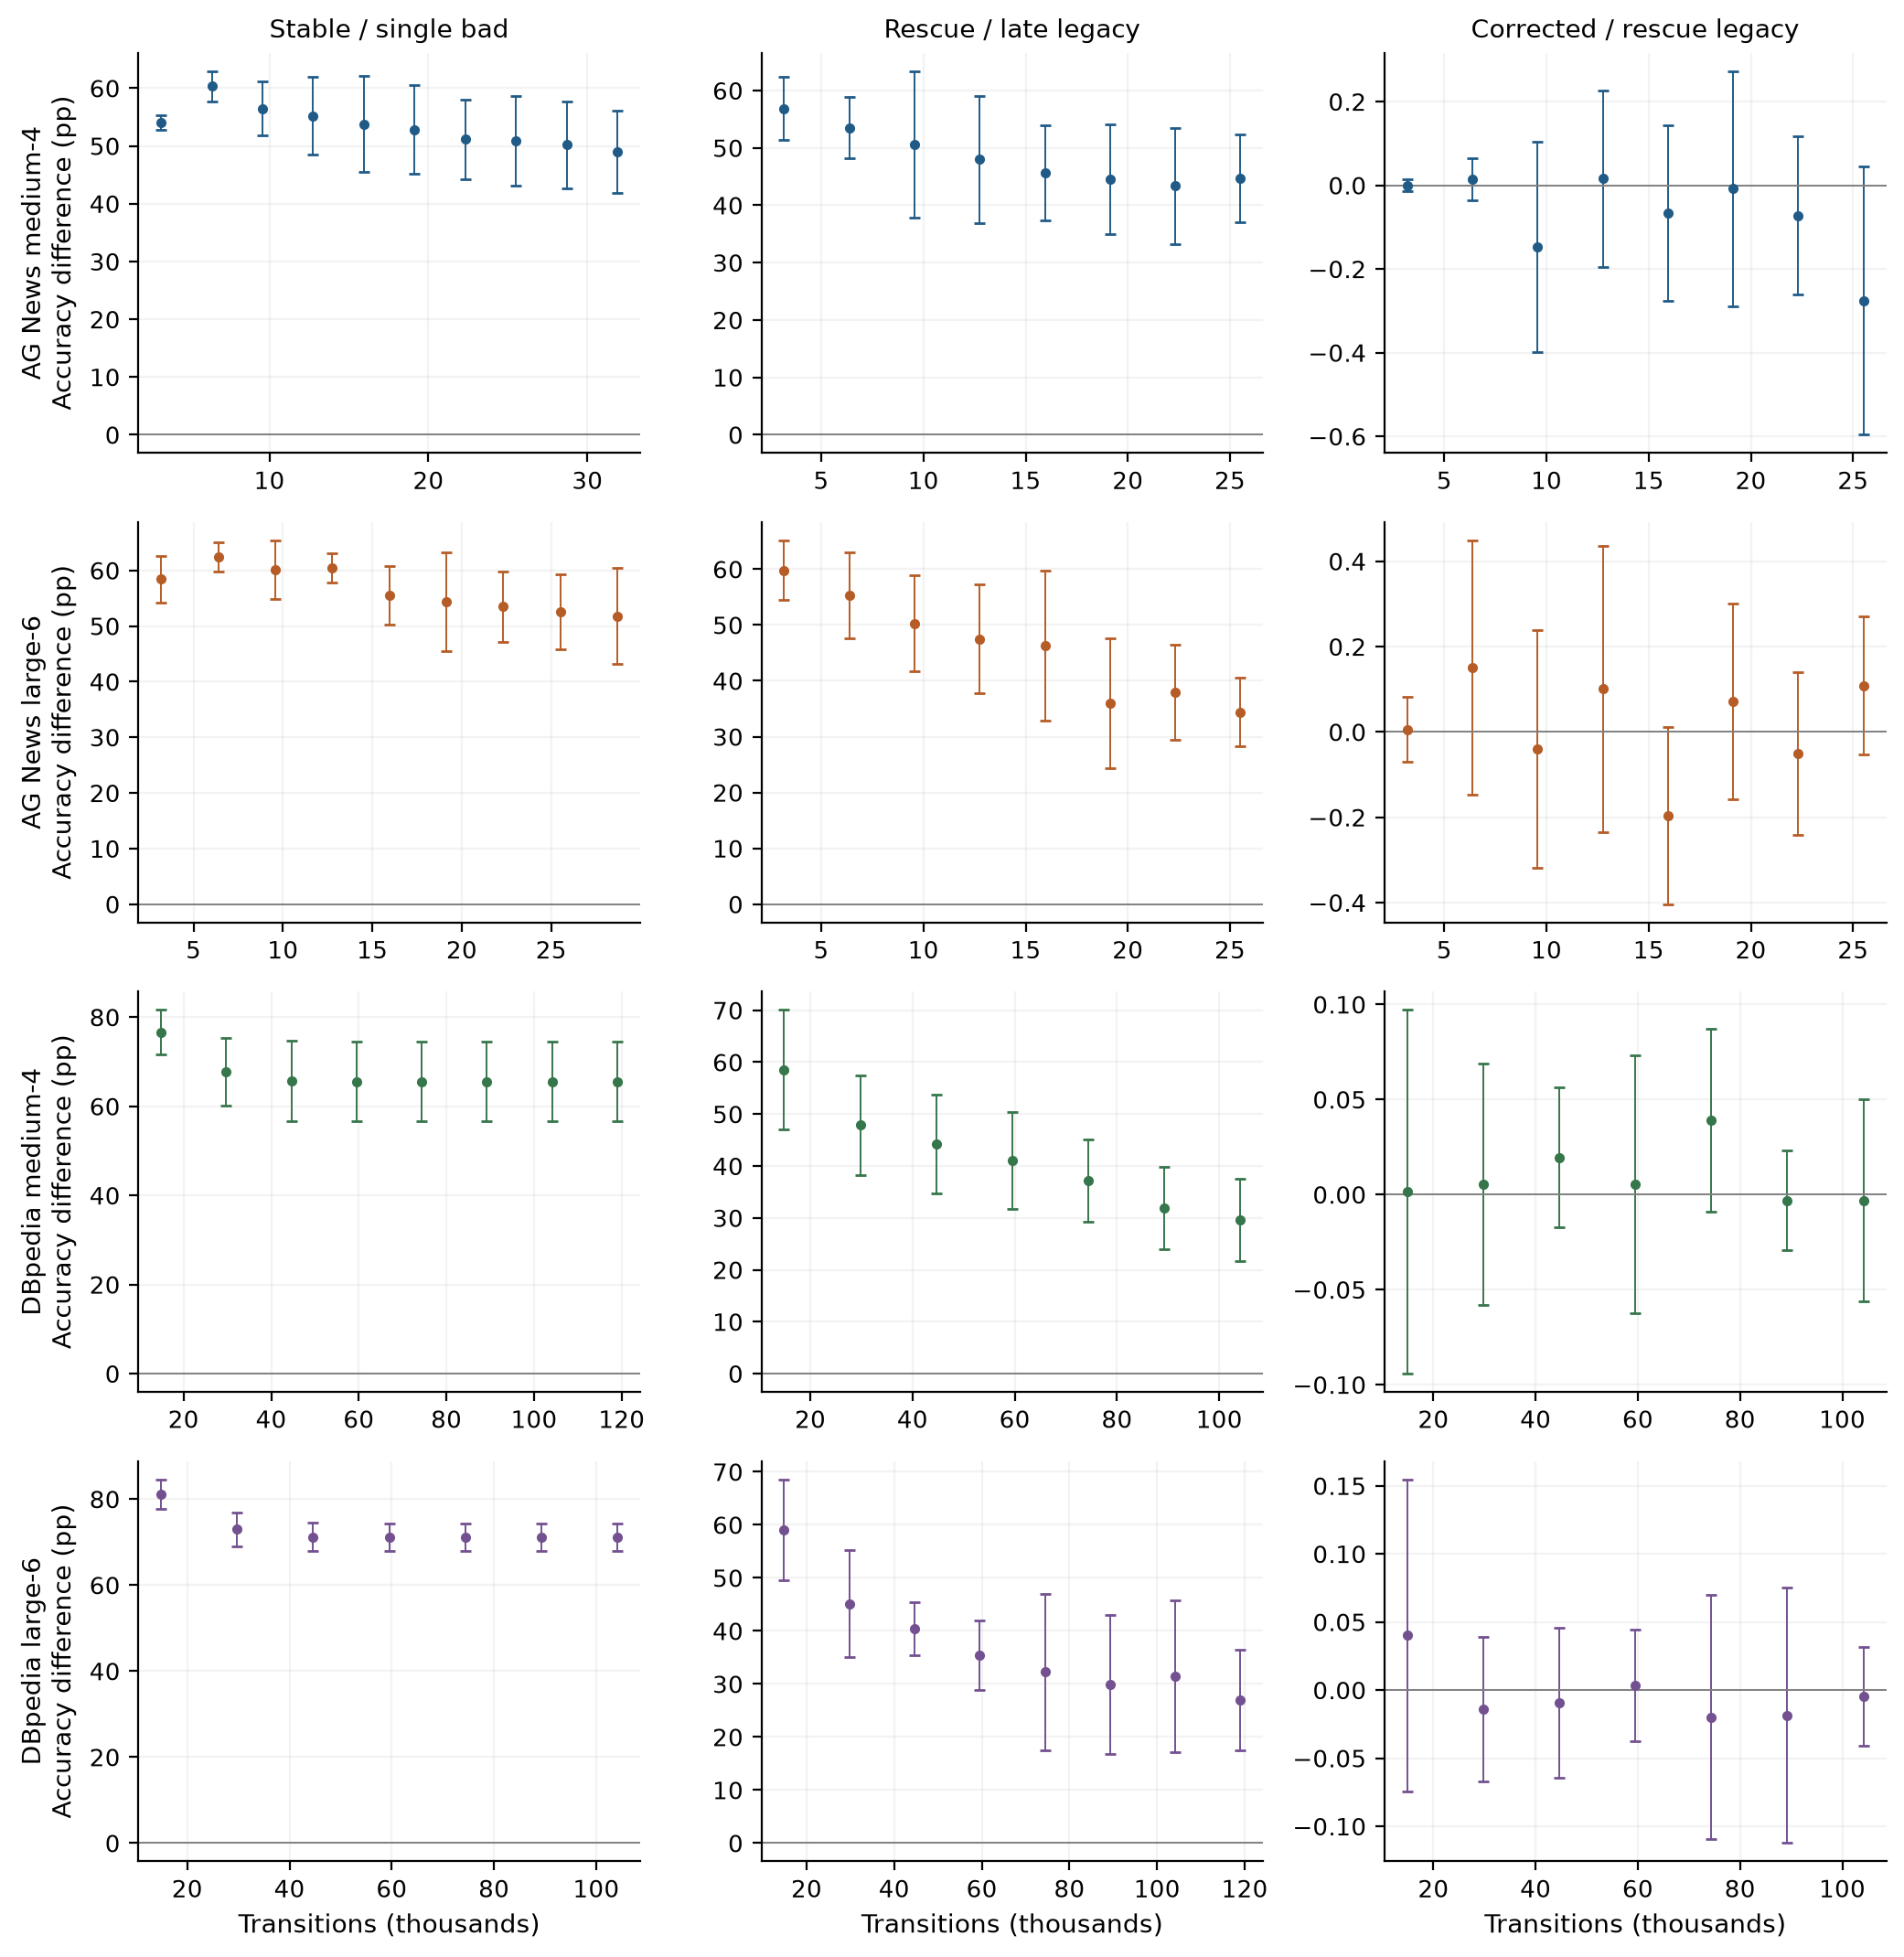
\includegraphics[width=0.98\linewidth,height=\textheight,keepaspectratio,height=0.72\textheight,keepaspectratio]{../figures/figS1_all_shared_step_paired_intervals.png}
\caption{All 95 paired shared-step validation accuracy differences with descriptive 95\% Student-t intervals, n=5. Each panel retains all shared logged steps and uses its own vertical scale.}
\end{figure}

\section{Supporting trajectories and provenance}\label{supporting-trajectories-and-provenance}

\begin{figure}[htbp]
\centering
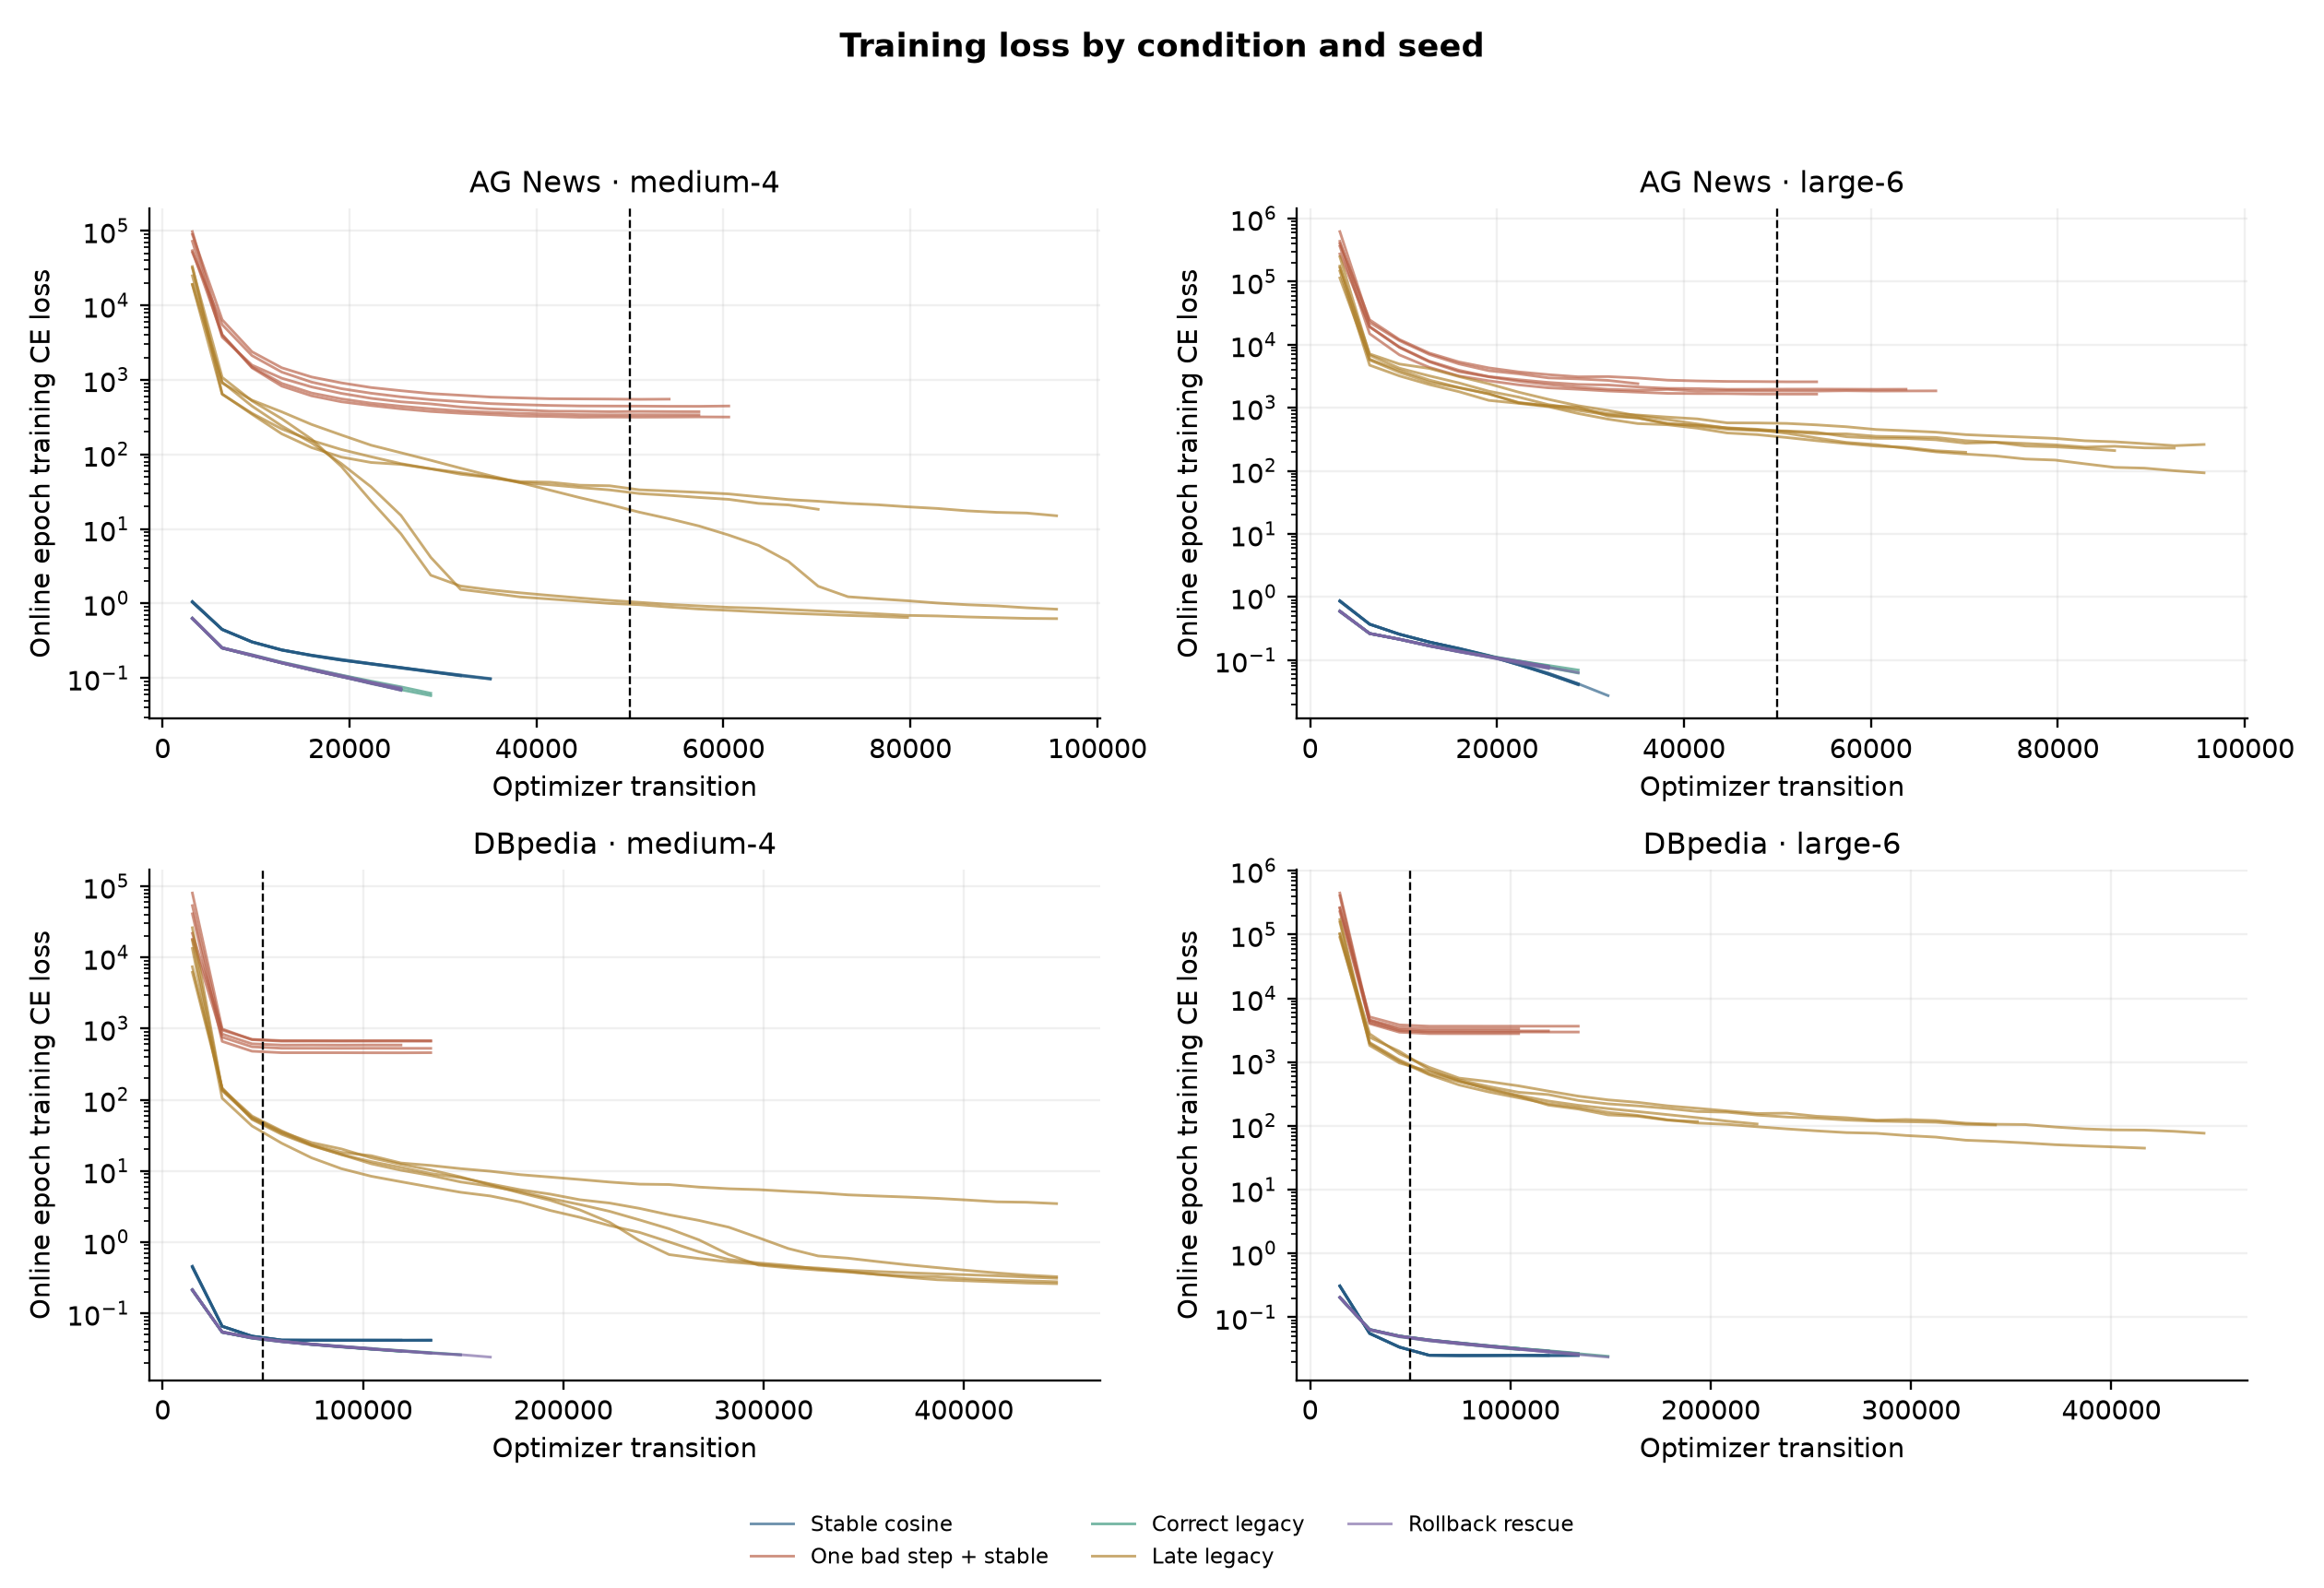
\includegraphics[width=0.95\linewidth,height=\textheight,keepaspectratio,height=0.72\textheight,keepaspectratio]{../figures/figS2_archived_online_training_loss.png}
\caption{Archived online training loss by condition, recorded while parameters and dropout state change. These trajectories are distinct from fixed-checkpoint validation evaluation.}
\end{figure}

\begin{figure}[htbp]
\centering
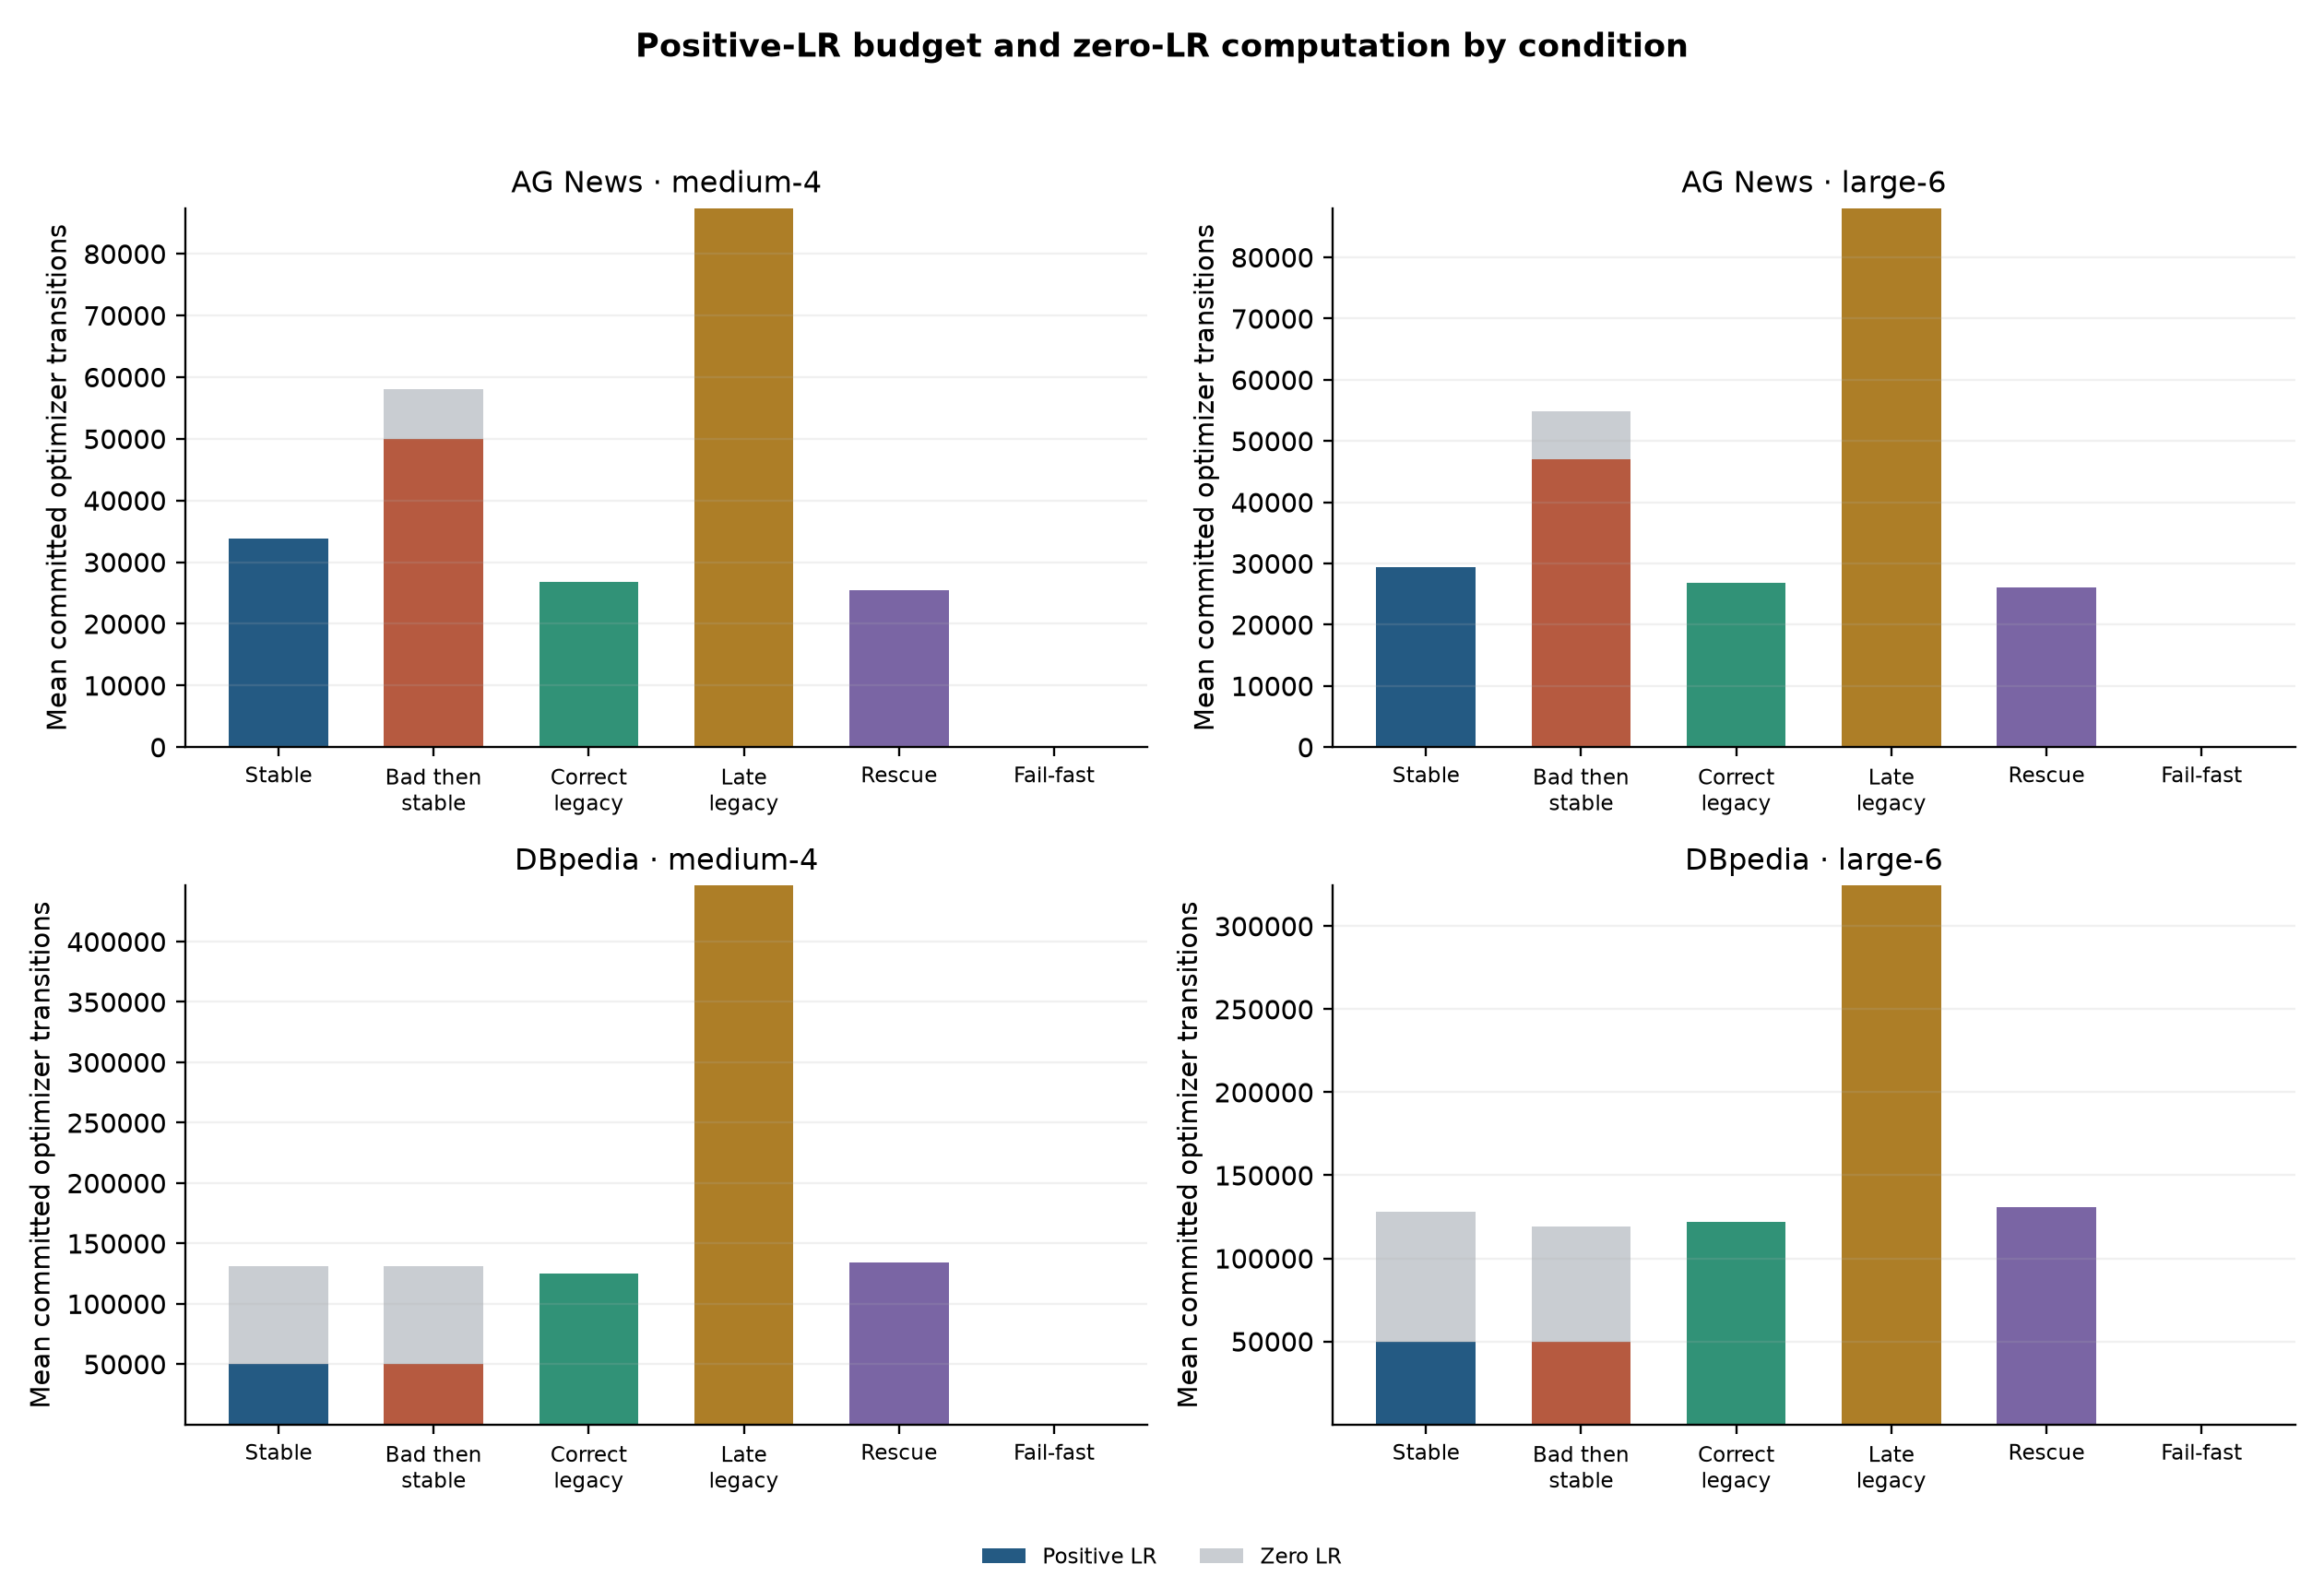
\includegraphics[width=0.95\linewidth,height=\textheight,keepaspectratio,height=0.72\textheight,keepaspectratio]{../figures/figS3_positive_and_zero_lr_budgets.png}
\caption{Positive-LR transitions, zero-LR computation and replay overhead remain separate.}
\end{figure}

\begin{figure}[htbp]
\centering
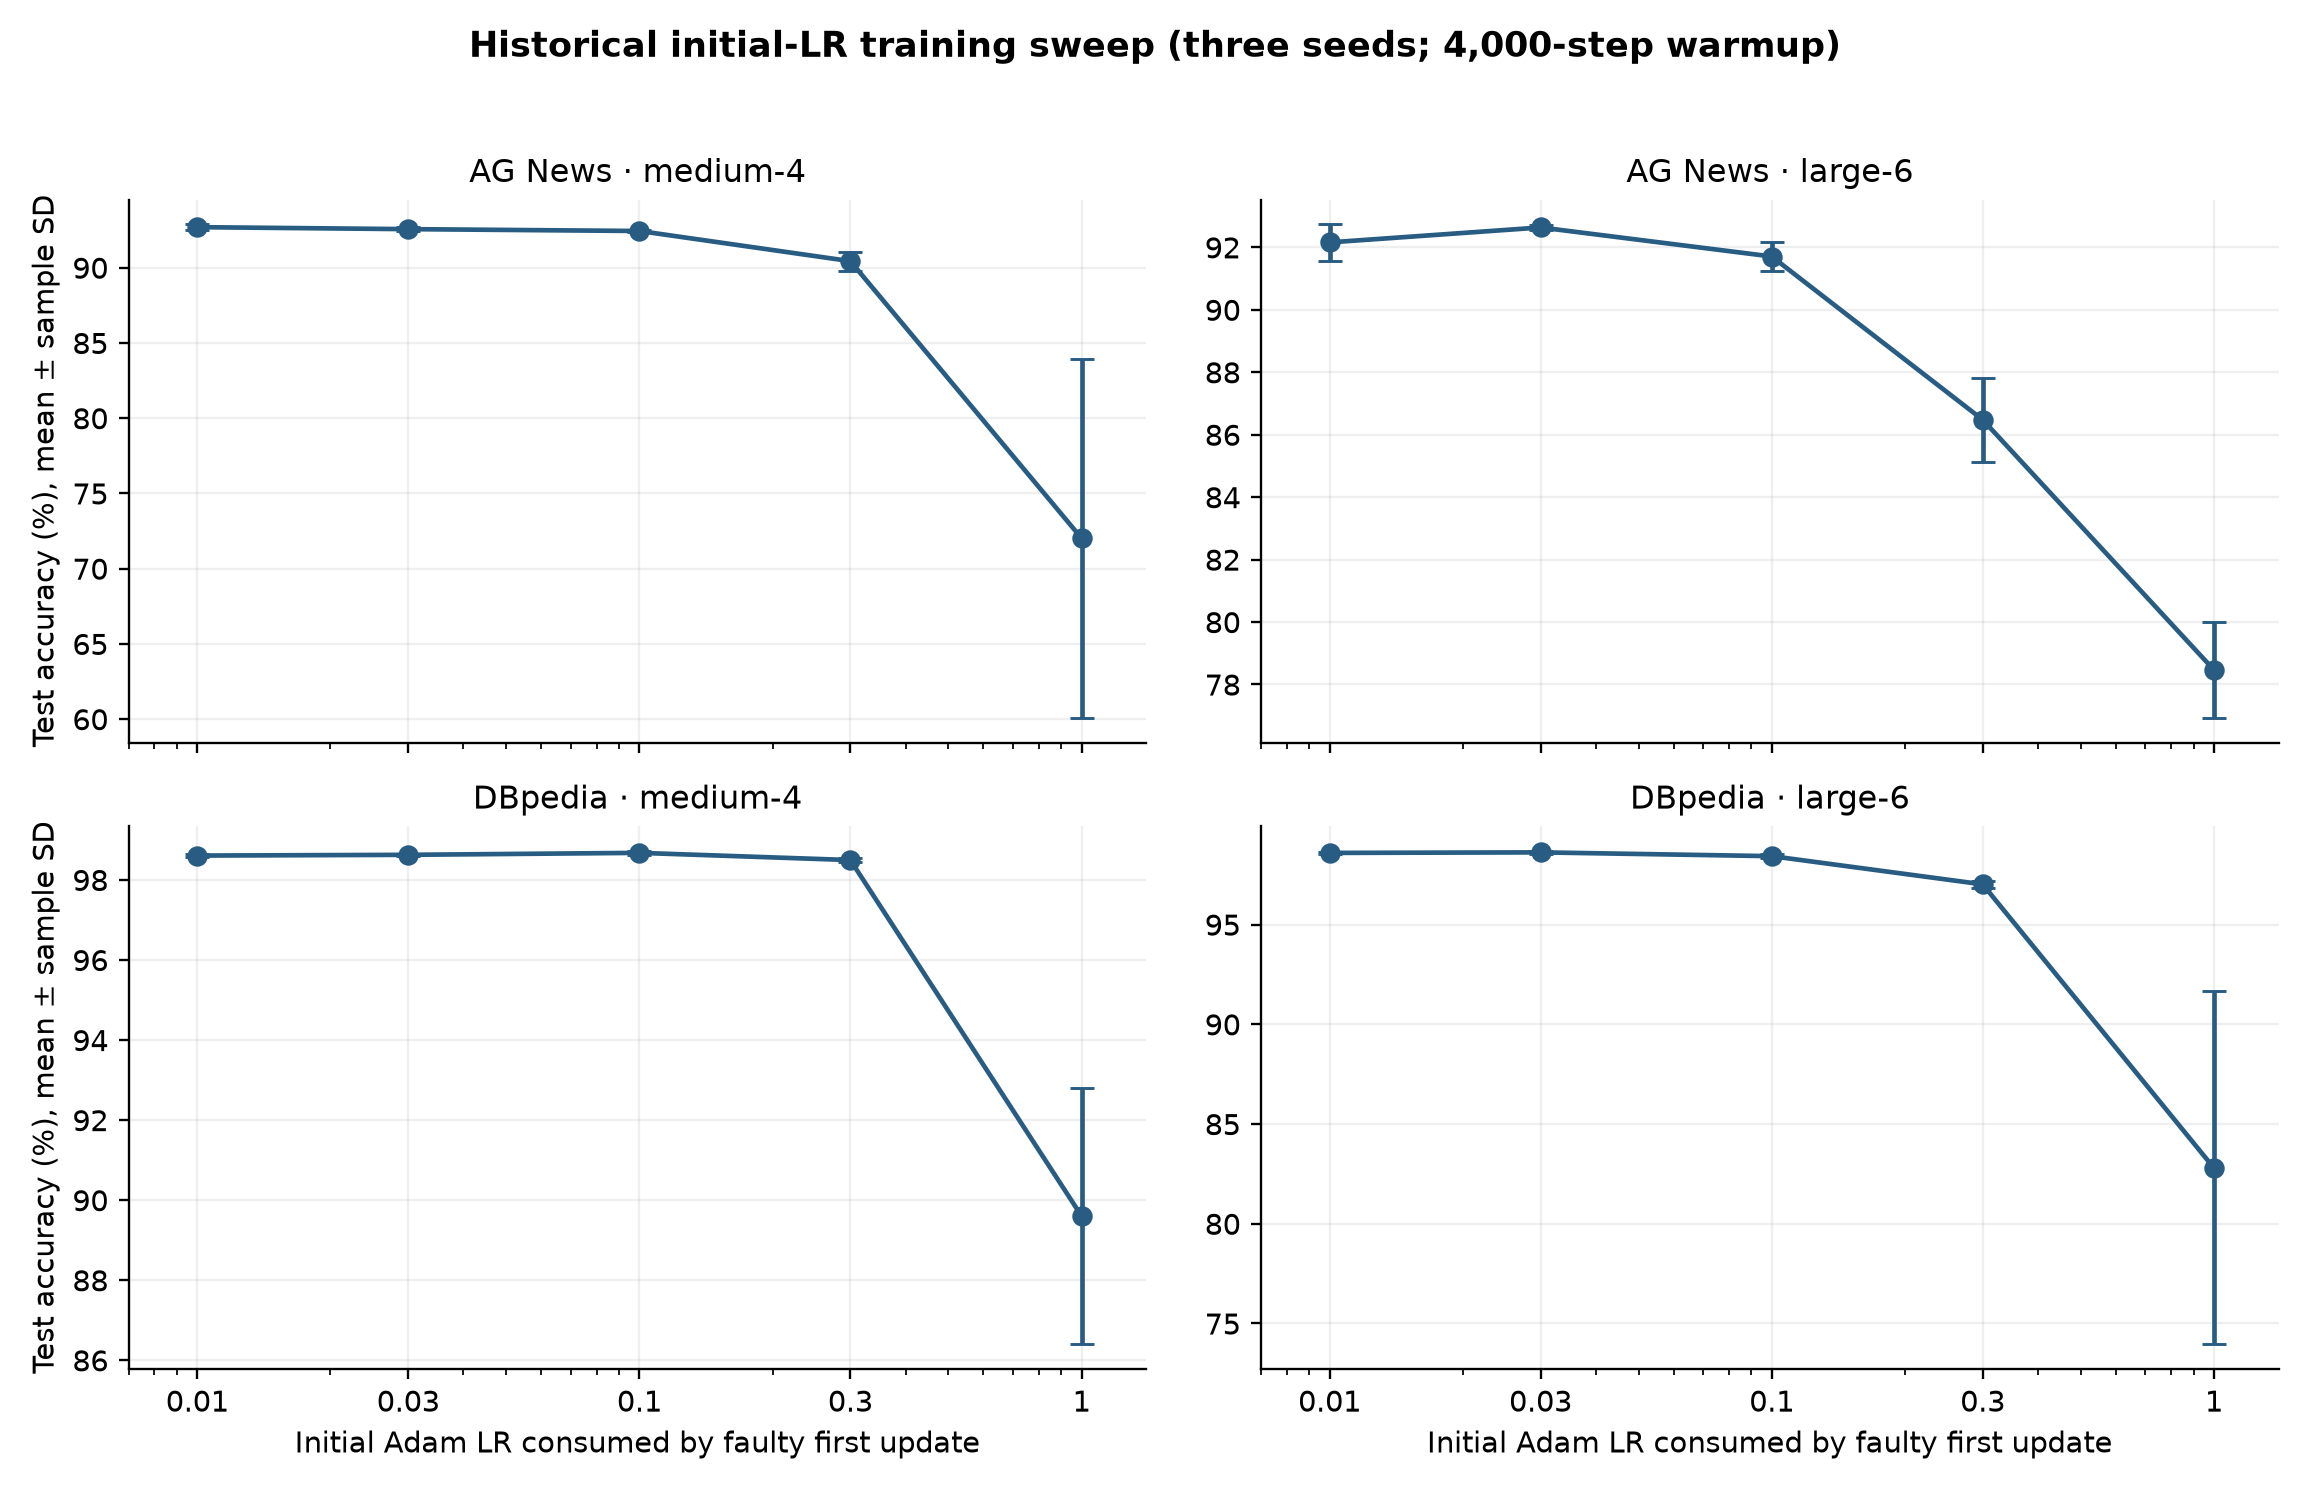
\includegraphics[width=0.95\linewidth,height=\textheight,keepaspectratio,height=0.72\textheight,keepaspectratio]{../figures/figS4_historical_initial_lr_severity.png}
\caption{Historical three-seed/W4000 trained-model severity outcomes; separate from October five-seed/W8000.}
\end{figure}

\begin{figure}[htbp]
\centering
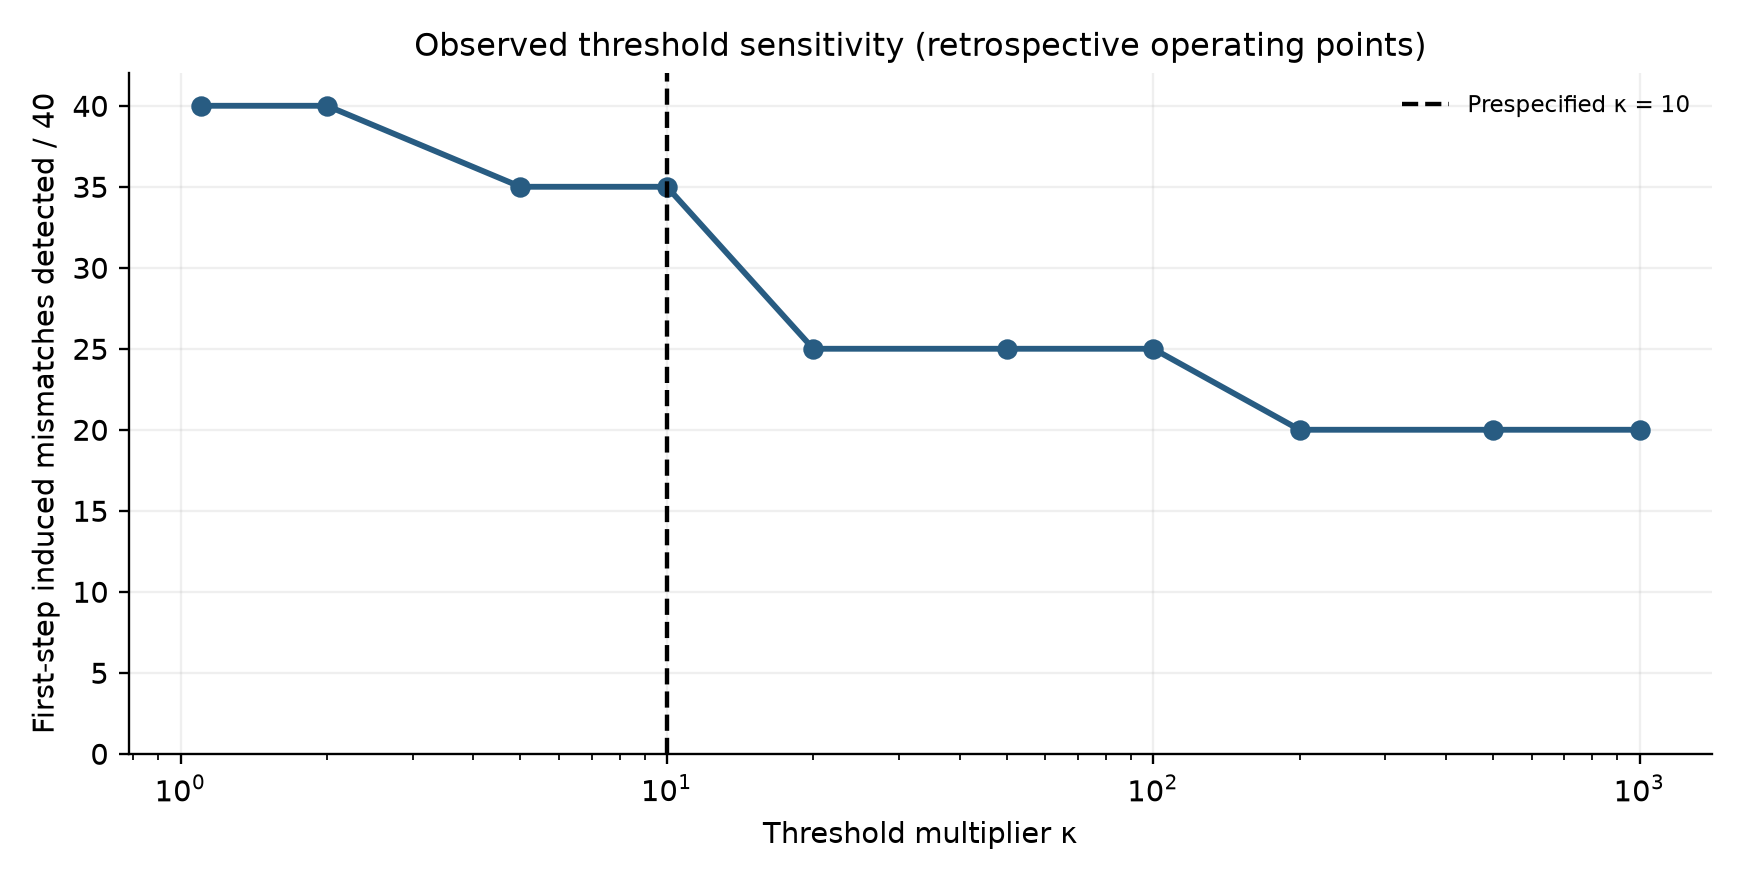
\includegraphics[width=0.95\linewidth,height=\textheight,keepaspectratio,height=0.72\textheight,keepaspectratio]{../figures/figS5_retrospective_threshold_sensitivity.png}
\caption{Primary kappa=10 and retrospective sensitivity; WNUT misses remain visible.}
\end{figure}

\begin{figure}[htbp]
\centering
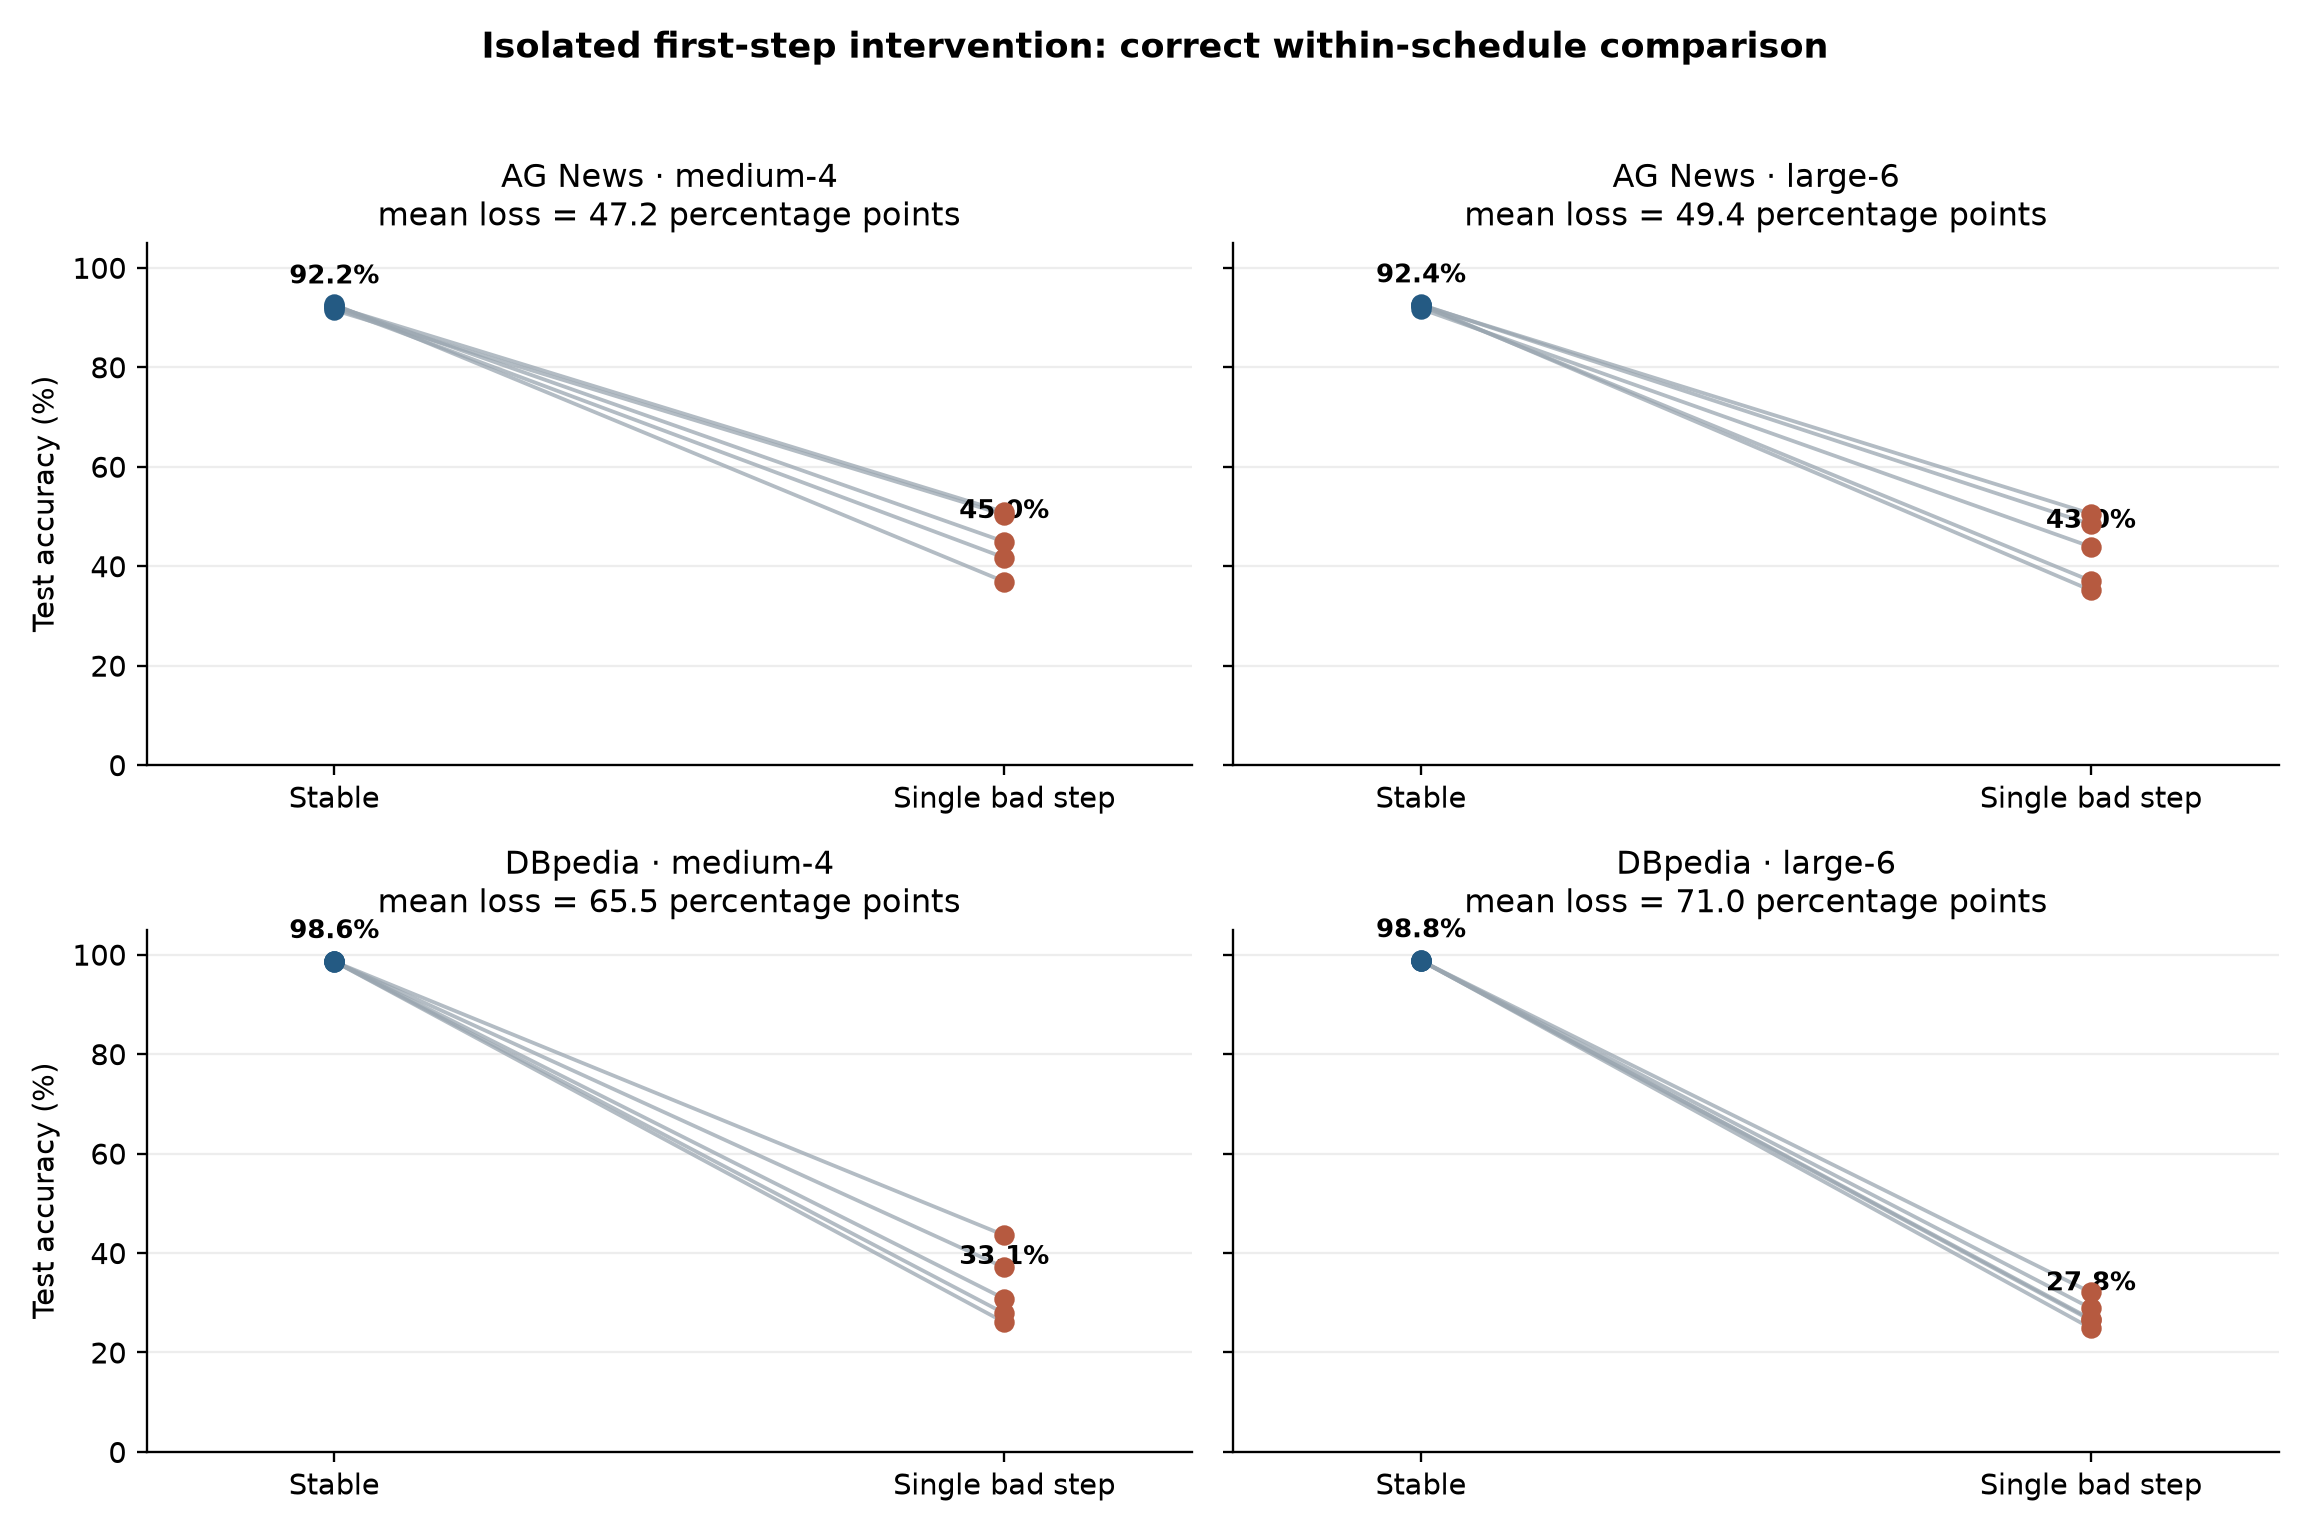
\includegraphics[width=0.95\linewidth,height=\textheight,keepaspectratio,height=0.72\textheight,keepaspectratio]{../figures/figS6_stable_bad_selected_endpoints.png}
\caption{All five stable and isolated-bad selected endpoints.}
\end{figure}

\begin{figure}[htbp]
\centering
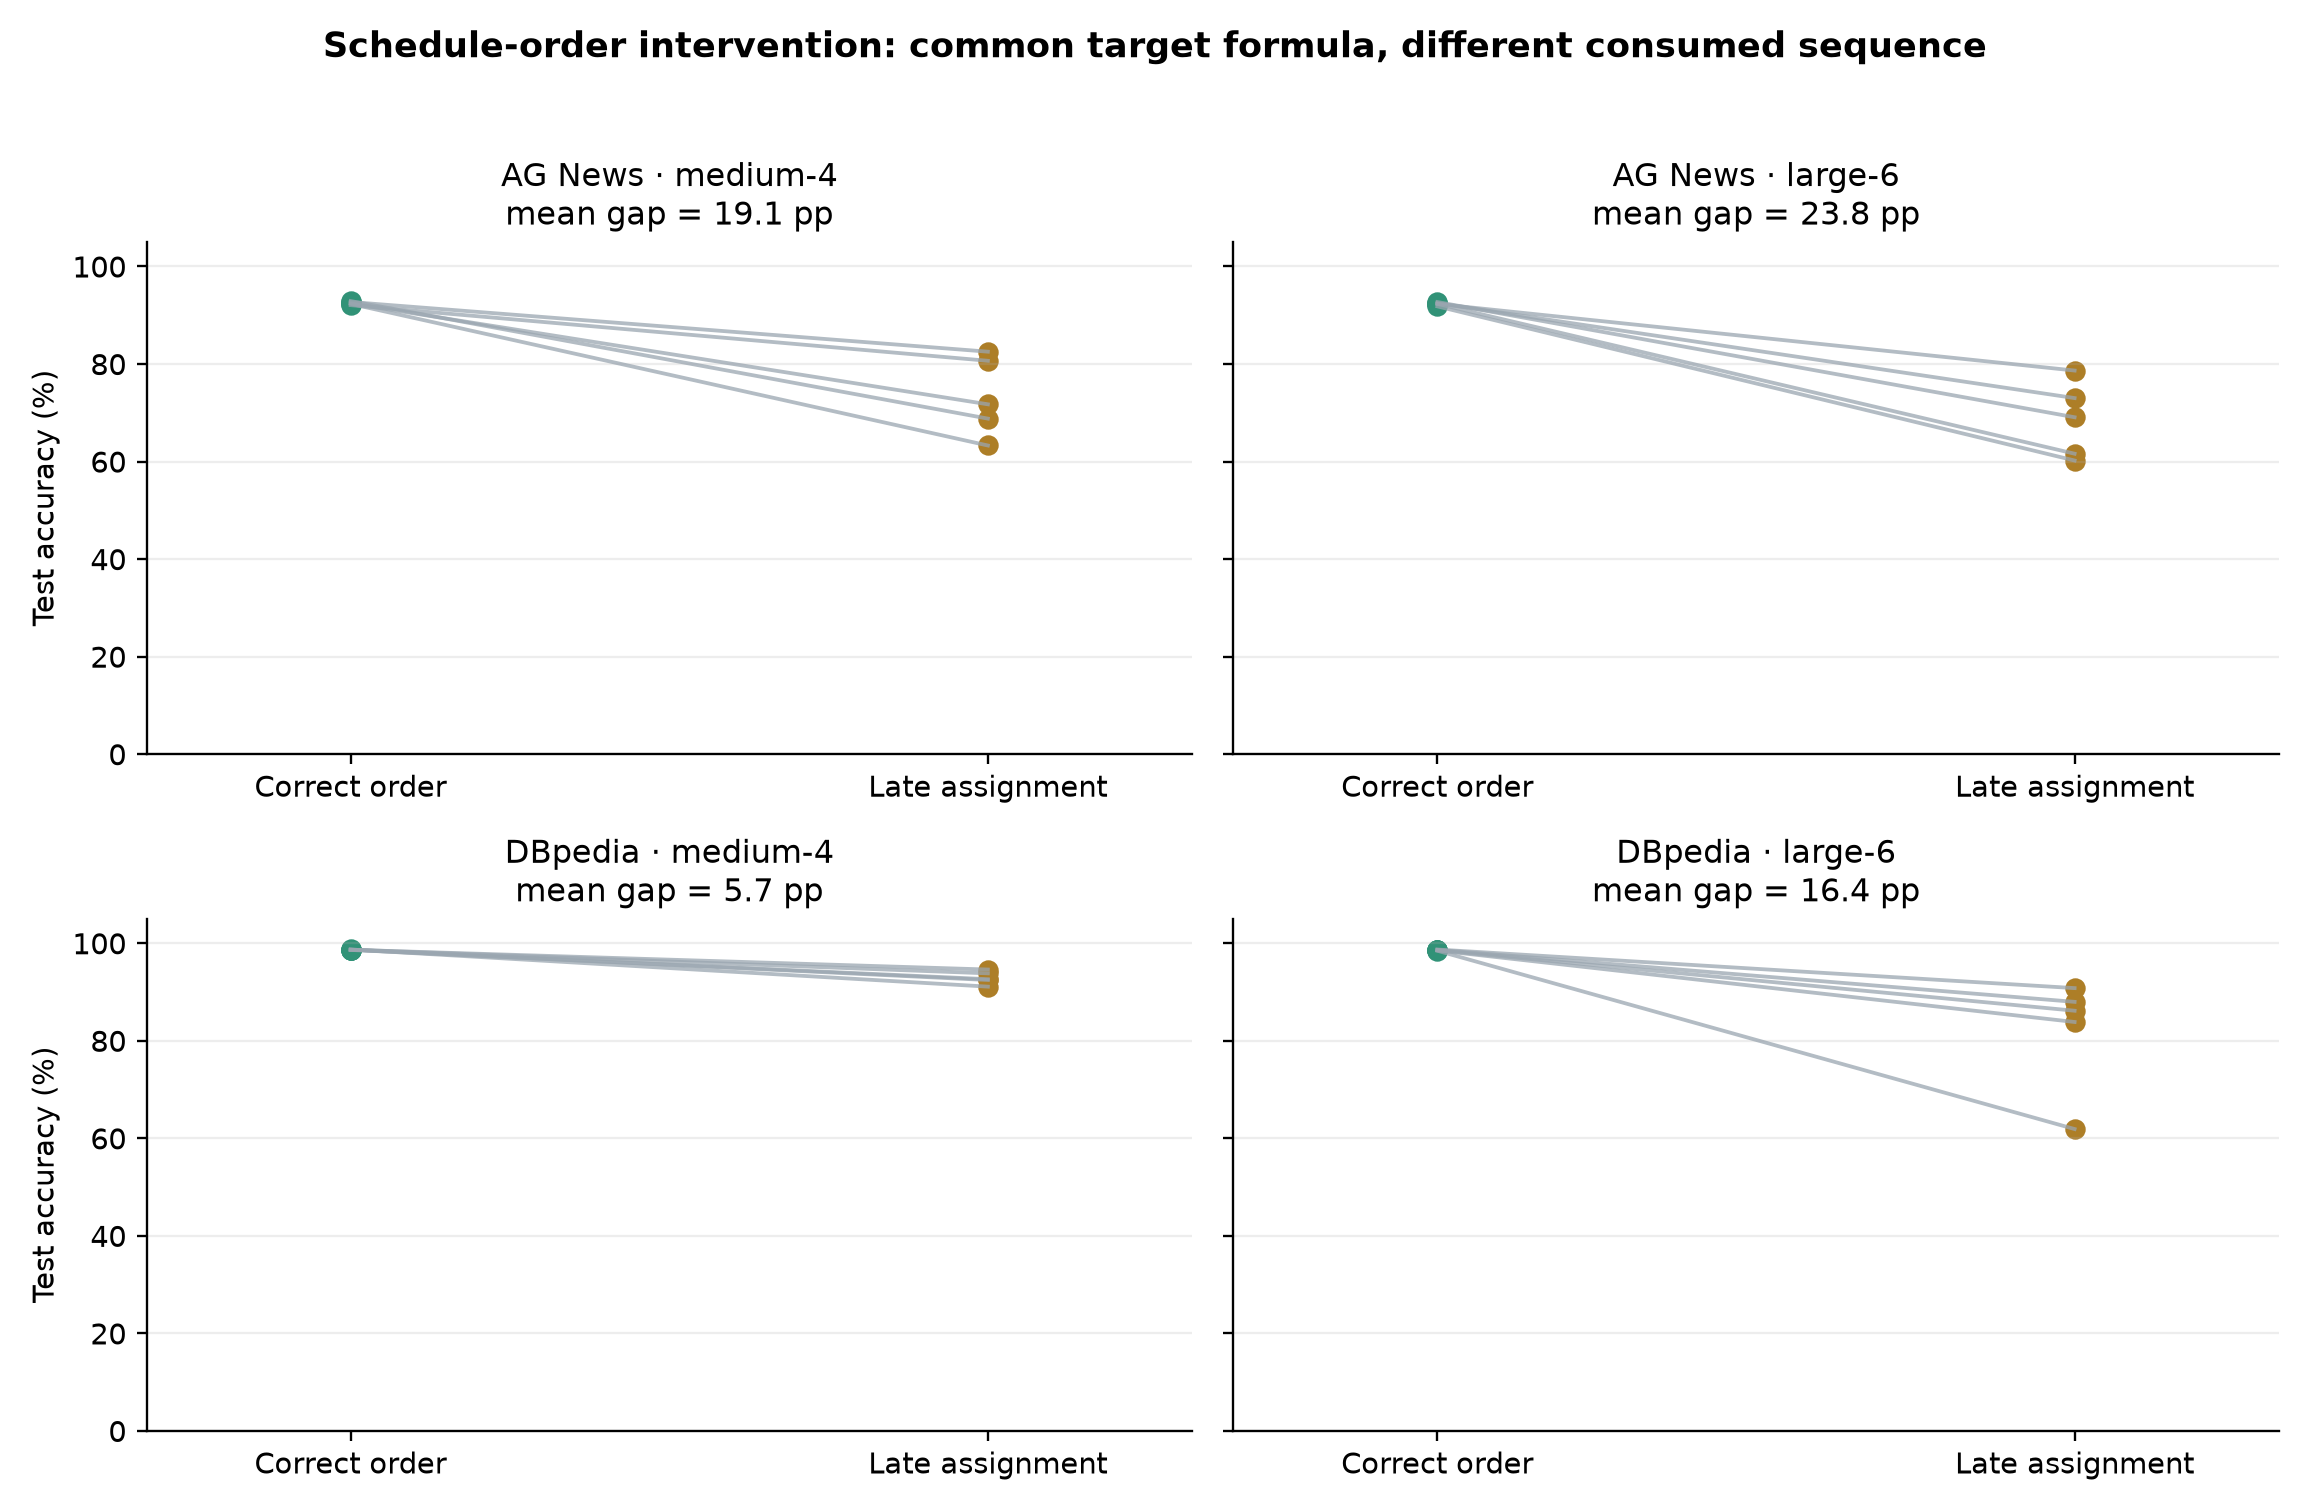
\includegraphics[width=0.95\linewidth,height=\textheight,keepaspectratio,height=0.72\textheight,keepaspectratio]{../figures/figS7_legacy_selected_endpoints.png}
\caption{All five corrected and late legacy selected endpoints; stopping budgets differ.}
\end{figure}

\begin{figure}[htbp]
\centering
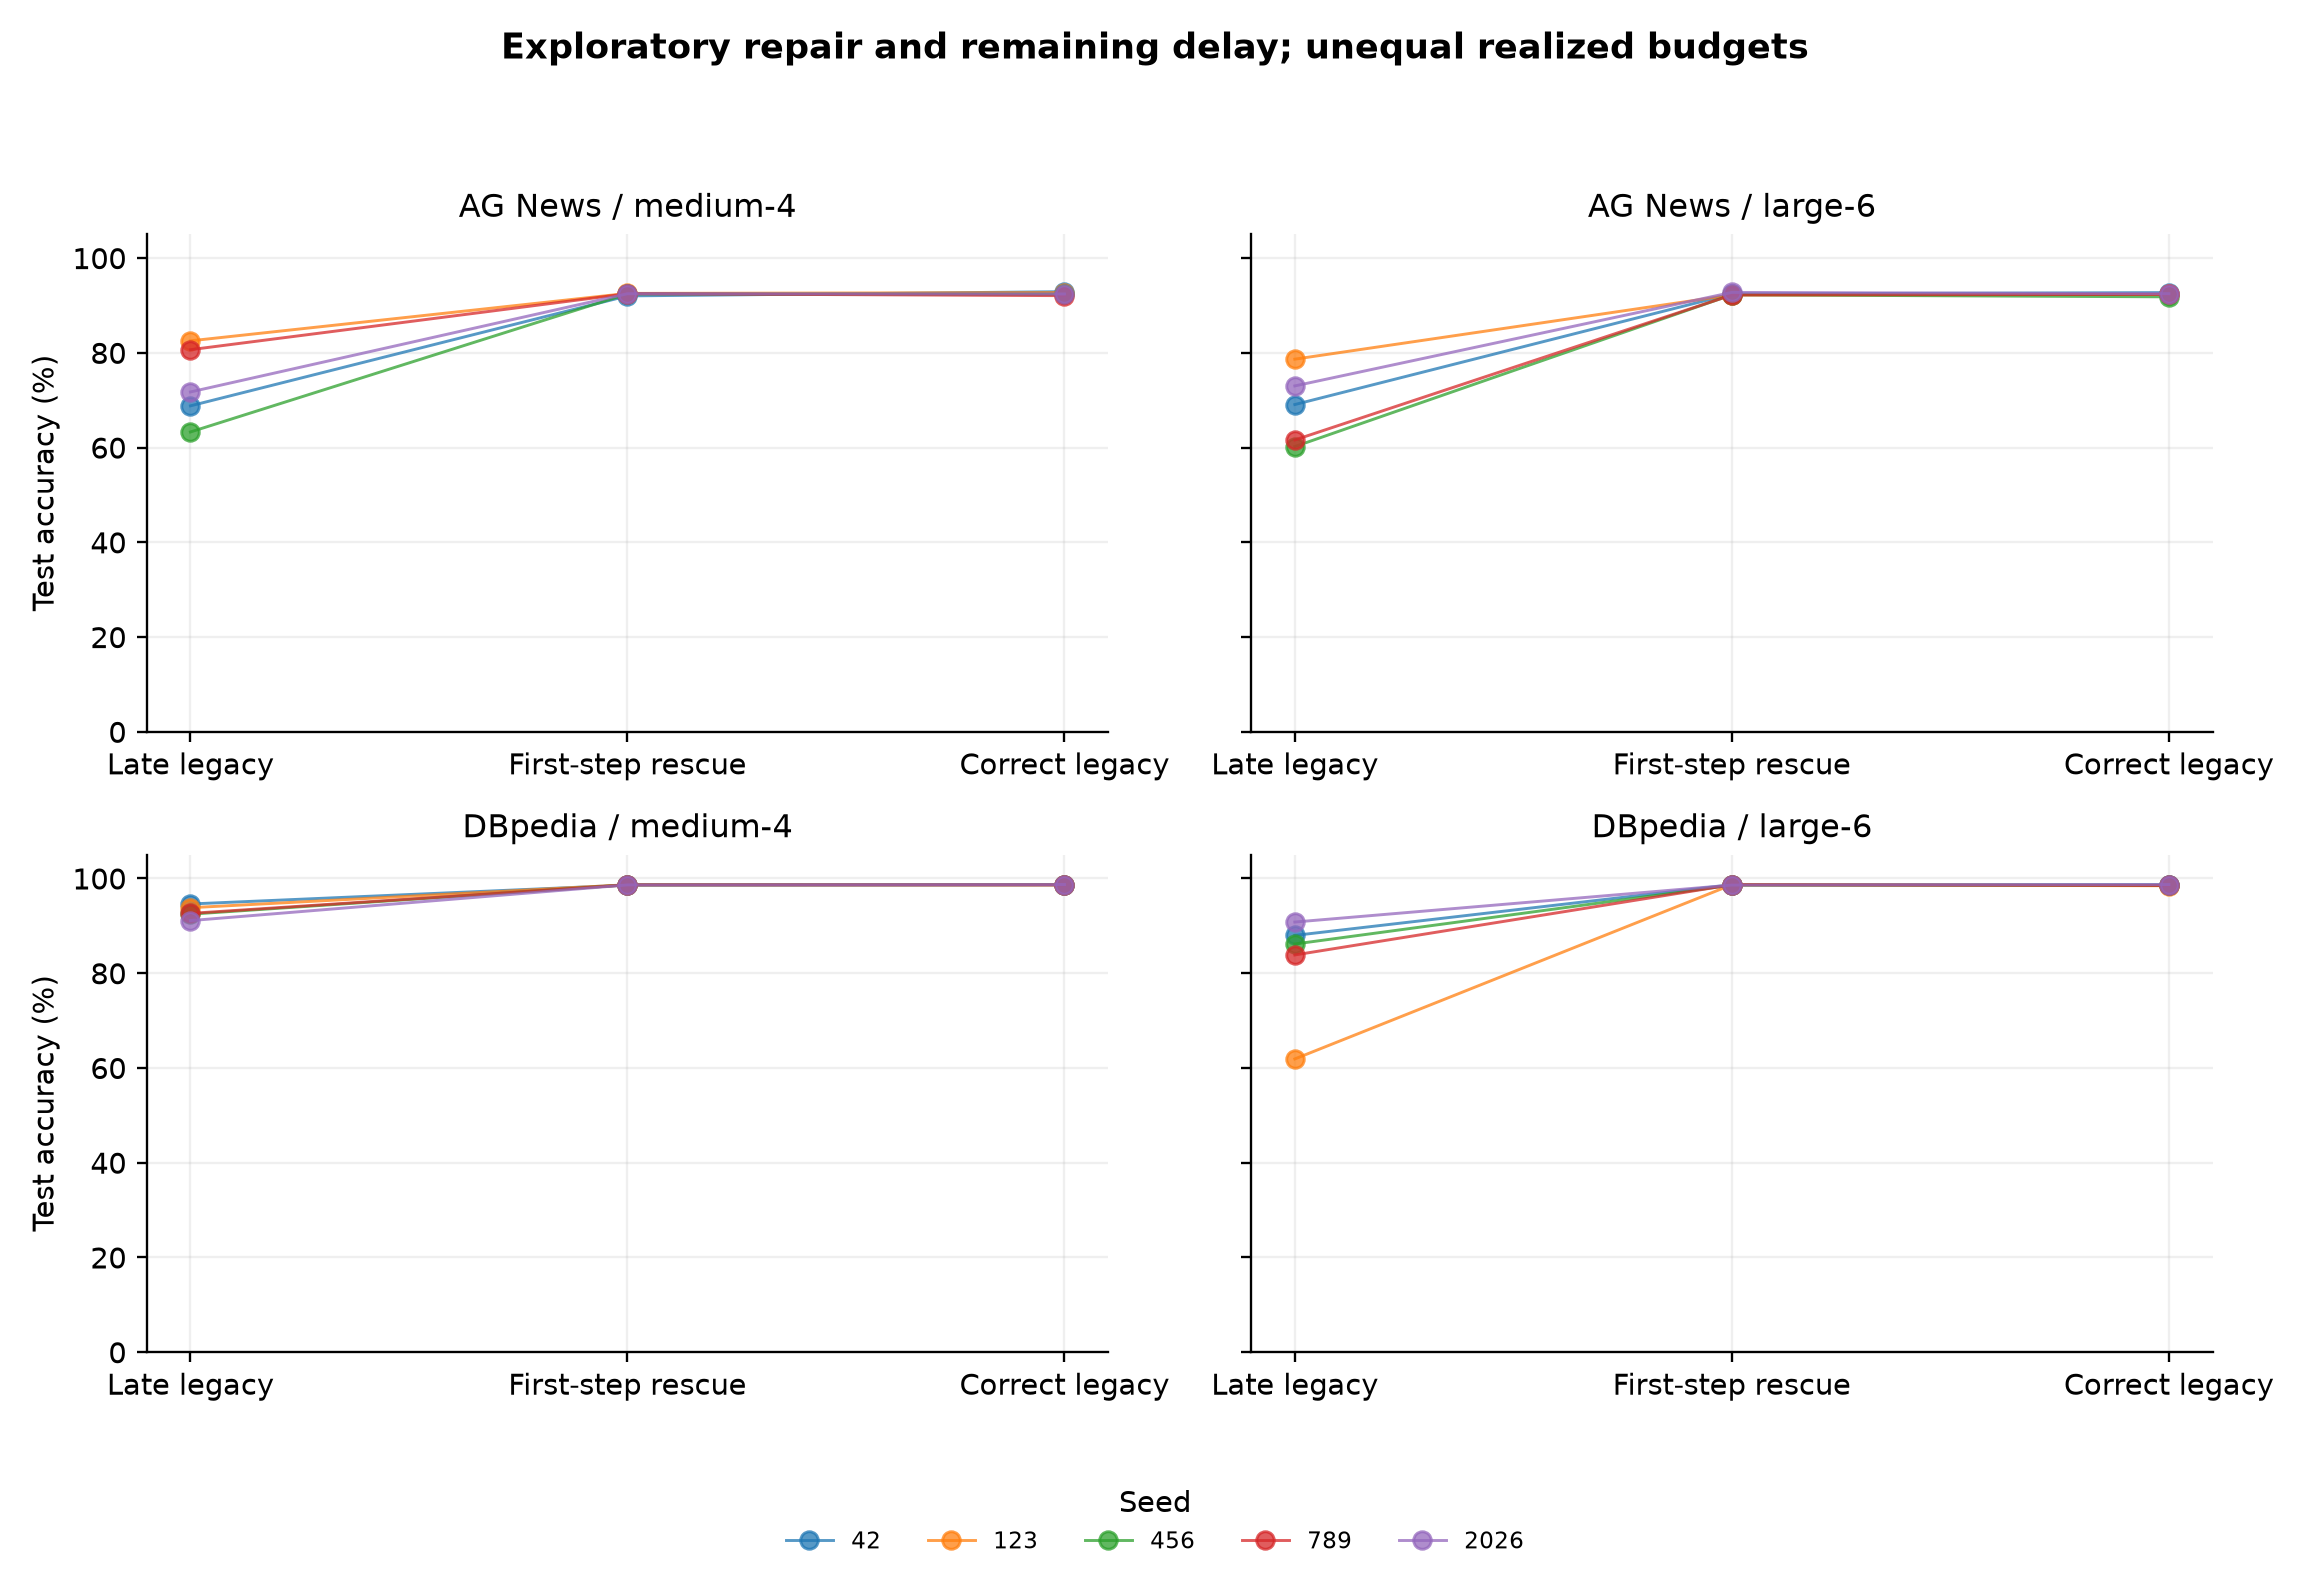
\includegraphics[width=0.95\linewidth,height=\textheight,keepaspectratio,height=0.72\textheight,keepaspectratio]{../figures/figS8_exploratory_legacy_endpoints.png}
\caption{Exploratory legacy selected endpoints; conditional comparisons do not complete a factorial.}
\end{figure}

\section{Historical configuration and analysis-reference provenance}\label{historical-configuration-and-analysis-reference-provenance}

The historical initial-LR sweep used buggy legacy scheduling with \textbf{4,000 warmup steps}, three seeds (42, 123, 456), two model sizes and five initial rates \(\{1,0.3,0.1,0.03,0.01\}\) per dataset (60 runs). Outcomes were extracted from preserved executed notebook tables. The notebook manifests omit warmup, but both original sweep runners explicitly pass warmup\_steps=4000 to ScratchTrainer, overriding its 8000-step default. All 30 complete AG News LR traces agree with the 4,000-step schedule and peak; the archived DBpedia first-step trace export agrees with its runner. Full DBpedia trajectories were not rechecked. We recompute sample SD from the per-seed outcomes because the notebook summaries used population SD. These results are reported separately from the five-seed October study with 8,000 warmup steps. The earlier fixed-gradient counterfactual at rates down to \(10^{-4}\) measures one transition, not trained-model outcomes.

The separate analysis reference now matches the runners: pretrained single-bad step 1 exits at its installed target LR, scratch single-bad step 1 exits at LR=1.0, and guard enforcement ends after step 100. Original training code and records are unchanged. The 80 missing threshold entries are exported from result JSON fields, and sensitivity tables are regenerated from the safe traces and LOSO manifests. Source mappings accompany main and supplementary tables.

\section{Evaluation fixtures and replay implementation details}\label{evaluation-fixtures-and-replay-implementation-details}

The extreme-logit CPU fixture gives logit CE 2000 versus clipped-probability NLL 27.631. A deliberately uneven 32-plus-1 fixture gives an archived batch-mean loss of 5.347 versus example-weighted 0.975. These fixtures demonstrate evaluator behavior, not the magnitude or checkpoint-ranking effect of the actual AG News final batch. The corrected evaluator is partition-invariant in the regression fixture.

\subsection{Archived fixed-gradient contract}\label{archived-fixed-gradient-contract}

Exact replay requires restoration of weights, Adam moments and step counters, parameter groups, and clipped gradients. The CPU tests compare the unchanged executor against a clean safe step using warmed Adam state. The candidate and replay reuse gradients computed before the snapshot; they do not repeat the stochastic forward pass. For this deterministic Adam step, Python, NumPy and PyTorch CPU RNG states remain unchanged. A separate test perturbs and restores those states and checks the next draws. The step snapshot itself does not contain RNG state. These checks cover fixed-gradient CPU replay, not stochastic optimizer steps, AMP, CUDA or distributed execution.

\subsection{Separately versioned finite-state contract}\label{separately-versioned-finite-state-contract}

Source inspection and tiny CPU counterexamples identify two executor limitations. A direct comparison \texttt{NaN\ \textgreater{}\ threshold} is false, so threshold comparison alone does not reject nonfinite updates. Replaying at the intended LR also need not enforce a displacement ceiling: a scalar Adam fixture gives a replay ratio near 0.100 with threshold 0.001. Neither failure was observed in the saved scientific traces, and these counterexamples do not explain historical training outcomes.

The versioned future executor checks finite gradients/model/optimizer state before the candidate, and finite parameters, buffers, moments, counters and ratios after updates. Numerical failure restores a verified finite snapshot and stops. A missing verified state is reported explicitly rather than described as successful repair. A nonfinite gradient is not repaired by changing the LR.

The new contract permits at most one same-gradient replay and revalidates it. A nonfinite or over-threshold replay is restored and rejected, with no committed transition. Threshold enforcement remains confined to steps 1-100; finite-state checks continue beyond that window. Regression fixtures cover steps 1, 100 and 101, warmed Adam state, and rejected replay accounting. The new fail-fast contract restores a rejected candidate; the archived fail-fast implementation retained its finite candidate before stopping. These versioned policies are not substituted into the historical evidence.

Separate full-boundary-state primitives retain RNG and sampler position. A tiny CPU dropout fixture reproduces uninterrupted execution after serialization and resume at a mid-permutation cursor. That check does not certify the original data-loader trajectory, actual training device, AMP or distributed recovery. These CPU fixtures are separate from the completed configured-peak pair and its actual-device/data resume check reported below; historical checkpoint-level prediction reevaluation remains unavailable.

\section{Execution provenance: design metadata and returned job outcomes}\label{execution-provenance-design-metadata-and-returned-job-outcomes}

Five negative completion flags in the master/dataset manifests are unchanged from the original pre-execution launcher. All 49 non-result JSON files in the returned package match the source launcher byte for byte. The flags are retained as historical metadata; job execution is evaluated from the accompanying result, status, job-manifest, history and transition records. Their identity and file digests are exported per run in \path{execution_provenance_per_run.csv}.

\begin{longtable}[]{@{}
  >{\raggedright\arraybackslash}p{(\linewidth - 6\tabcolsep) * \real{0.2500}}
  >{\raggedright\arraybackslash}p{(\linewidth - 6\tabcolsep) * \real{0.2500}}
  >{\raggedleft\arraybackslash}p{(\linewidth - 6\tabcolsep) * \real{0.2500}}
  >{\raggedleft\arraybackslash}p{(\linewidth - 6\tabcolsep) * \real{0.2500}}@{}}
\toprule\noalign{}
\begin{minipage}[b]{\linewidth}\raggedright
Cohort
\end{minipage} & \begin{minipage}[b]{\linewidth}\raggedright
Recorded termination
\end{minipage} & \begin{minipage}[b]{\linewidth}\raggedleft
Records
\end{minipage} & \begin{minipage}[b]{\linewidth}\raggedleft
Trained test endpoints
\end{minipage} \\
\midrule\noalign{}
\endhead
\bottomrule\noalign{}
\endlastfoot
Scratch & Early stopping & 89 & 89 \\
Scratch & Maximum epochs & 11 & 11 \\
Scratch & Guard fail-fast & 20 & 0 \\
Pretrained & Three epochs, ordinary training arms & 80 & 80 \\
Pretrained & Three epochs, WNUT fail-fast arms whose guard did not trigger & 5 & 0 \\
Pretrained & Guard fail-fast & 15 & 0 \\
Pretrained & LR assertion before mutation & 20 & 0 \\
\end{longtable}

Thus 240 scientific records contain 180 trained test endpoints. The five WNUT diagnostic arms do not become additional test classifiers merely because their guard missed and training continued. Twenty separate pretrained severity records are not added to this matrix.

The source comparison covers 224 byte-identical scientific Python/configuration copies in the original launcher, representing 56 distinct files across four dataset copies. All 1,573 saved history rows and 55,535 trace rows are checked against their job records; 277,675 LR fields match independently reconstructed schedules. All seven fingerprint fields match in each of 40 initialization groups. The two scratch dataset split manifests are identical across their respective 60 jobs. These checks establish consistency of saved evidence with the preserved implementation. They do not prove the final host executed unmodified source, reconstruct unavailable model states, or establish an exact training rerun.

The separate AG News log has 1,499 lines. Its 635 rounded epoch entries and 40 completion reasons agree with the returned scratch histories. Two queue-handling failures precede successful phases; a later cross-dataset threshold lookup error interrupts the guarded-phase launch. The log is therefore partial. The recovered 11 October hotfix unwraps queued job tuples and scopes the matrix enumerators to the current dataset before threshold lookup. Applying its pure text transformation to the original four launchers in memory produces syntactically valid, idempotent corrections without modifying scientific modules or results. These reconstructed wrappers explain the supplied repair but are not recovered execution-time files. Final patch-application logs, complete master status and console logs for other phases remain unavailable. The original environment files are design records, not an independently captured final host dependency lock.

The original scratch runner saves a rolling epoch-end resume state and overwrites its validation-best state. It deletes both temporary files after normal completion. This retention policy is consistent with their absence from returned results; it does not establish whether manual backups survive. No eligible candidate-epoch weights, matching validation predictions or full paired states immediately after transition 49,999 were recovered.

\section{Executable first-two-step and zero-LR examples}\label{executable-first-two-step-and-zero-lr-examples}

The supplied example uses three float64 CPU parameters and two fixed clipped gradients. It imports the frozen scratch runner's condition policy, model-specific schedule and Adam constructor, and instruments actual optimizer calls. It has no dataset input. The threshold used to illustrate rescue is a fixture value, not a new research calibration.

\begin{longtable}[]{@{}
  >{\raggedright\arraybackslash}p{(\linewidth - 4\tabcolsep) * \real{0.3333}}
  >{\raggedright\arraybackslash}p{(\linewidth - 4\tabcolsep) * \real{0.3333}}
  >{\raggedright\arraybackslash}p{(\linewidth - 4\tabcolsep) * \real{0.3333}}@{}}
\toprule\noalign{}
\begin{minipage}[b]{\linewidth}\raggedright
Condition
\end{minipage} & \begin{minipage}[b]{\linewidth}\raggedright
Actual LR calls at transition 1
\end{minipage} & \begin{minipage}[b]{\linewidth}\raggedright
Actual LR calls at transition 2
\end{minipage} \\
\midrule\noalign{}
\endhead
\bottomrule\noalign{}
\endlastfoot
Stable & S(1) & S(2) \\
Single bad then stable & 1.0 & S(2) \\
Corrected legacy & L(1) & L(2) \\
Late legacy & 1.0 & L(1) \\
Legacy rescue & 1.0 rejected, then L(1) replayed & L(1) \\
Archived fail-fast & 1.0, retained before stop & No transition \\
LR assertion & No optimizer call & No transition \\
\end{longtable}

For widths 128 and 256, the example observes both the candidate and replay calls. The replay restores the initial Adam counter before updating, so two calls at the first transition leave one committed step. Its retained state matches a clean legacy first transition. At transition two the rescued arm still consumes L(1); correction of the first transition did not remove later lag. The scratch isolated-fault arm exits transition one with stored LR=1.0, then installs S(2) before its next update.

The assertion rejects before mutation. Its archived result field named candidate\_lr holds the entry value even though no optimizer call consumed that value; the example reports no actual consumed LR. A separate three-update fixture installs S(50,000)=0 on its last call. Parameters remain unchanged while both Adam moment arrays and the counter change. This is a boundary-value fixture, not a recovered or newly trained 49,999-step state.

\section{Reproduction scope}\label{reproduction-scope}

The supplied analyses reconstruct tables and figures from the preserved result archive and historical notebook exports. The reproducibility command also checks unchanged source/data digests, original scientific CSVs, displayed results, shared-step arithmetic, evaluator behavior and rollback fixtures. Original inputs are preserved separately from derived outputs.

The updated package adds the record-provenance audit and actual optimizer-call example. Its execution logs, commands, dependency versions and file digests accompany the sources. Saved-record analysis, CPU fixtures and typesetting are reproducible separately from original model training. The new fixed-budget configured-peak pair is reported separately below, including all saved predictions and full retained states. Historical checkpoint selections are unchanged; historical candidate-epoch assets remain unavailable. Full extreme-fault recovery remains unperformed.

\section{Completed configured-peak pair: design and evidence}\label{completed-configured-peak-pair-design-and-evidence}

One DBpedia medium-4 pair, seed 42 and split seed 42, was run with the prespecified 49,999-positive-update budget. The only first-transition rate change is from 1.25e-8 to 1e-4; rates at every later transition match exactly within the pair. Adam uses betas (0.9, 0.98), epsilon 1e-9, no weight decay and gradient norm clipping at 1. Both FP32 arms process 1,599,968 examples, with no early stopping, checkpoint selection, zero-LR transitions, guard rescue or recovery extension. The fixed sample-weighted validation CE contrast is primary; test metrics are evaluated only after the final states exist. The same 8,192 training examples form the checkpoint monitor subset.

The pinned DBpedia revision is 9abd46cf7fc8b4c64290f26993c540b92aa145ac. The archived split arrays reproduce the fixed 476,000/84,000 development partition and 70,000 official test identities. The prospective sampler's explicit permutation/cursor implementation is separate from the historical loader. All seven first-transition fingerprints match; full initial model states match; first-step Adam moments match while parameter states differ. Both RNG streams remain matched at every retained checkpoint.

\Needspace{16\baselineskip}

\section{Table S18 Complete validation trajectory for the configured-peak pair}\label{table-s18-complete-validation-trajectory-for-the-configured-peak-pair}

The ten evaluation times were fixed before execution. Accuracy differences below are peak-first minus clean; the primary CE difference has the same sign convention. No favorable horizon is selected.

\begin{longtable}[]{@{}
  >{\raggedleft\arraybackslash}p{(\linewidth - 10\tabcolsep) * \real{0.1667}}
  >{\raggedleft\arraybackslash}p{(\linewidth - 10\tabcolsep) * \real{0.1667}}
  >{\raggedleft\arraybackslash}p{(\linewidth - 10\tabcolsep) * \real{0.1667}}
  >{\raggedleft\arraybackslash}p{(\linewidth - 10\tabcolsep) * \real{0.1667}}
  >{\raggedleft\arraybackslash}p{(\linewidth - 10\tabcolsep) * \real{0.1667}}
  >{\raggedleft\arraybackslash}p{(\linewidth - 10\tabcolsep) * \real{0.1667}}@{}}
\toprule\noalign{}
\begin{minipage}[b]{\linewidth}\raggedleft
Step
\end{minipage} & \begin{minipage}[b]{\linewidth}\raggedleft
Clean CE
\end{minipage} & \begin{minipage}[b]{\linewidth}\raggedleft
Peak-first CE
\end{minipage} & \begin{minipage}[b]{\linewidth}\raggedleft
CE difference
\end{minipage} & \begin{minipage}[b]{\linewidth}\raggedleft
Clean accuracy (\%)
\end{minipage} & \begin{minipage}[b]{\linewidth}\raggedleft
Peak-first accuracy (\%)
\end{minipage} \\
\midrule\noalign{}
\endhead
\bottomrule\noalign{}
\endlastfoot
0 & 3.051259363 & 3.051259363 & +0 & 7.1238 & 7.1238 \\
1 & 3.051226574 & 2.872099949 & -0.179127 & 7.1226 & 6.8857 \\
100 & 2.920109288 & 2.805125819 & -0.114983 & 7.3417 & 7.0405 \\
1000 & 2.106699977 & 2.101909795 & -0.00479018 & 40.5595 & 40.8036 \\
8000 & 0.123956156 & 0.124018987 & +6.28318e-05 & 96.7524 & 96.7512 \\
10000 & 0.108207223 & 0.108012674 & -0.000194549 & 97.1810 & 97.1857 \\
20000 & 0.074079209 & 0.074229176 & +0.000149967 & 98.1857 & 98.1821 \\
30000 & 0.063660947 & 0.063634032 & -2.6915e-05 & 98.4071 & 98.4048 \\
40000 & 0.062740690 & 0.062726095 & -1.45951e-05 & 98.4964 & 98.4988 \\
49999 & 0.061363441 & 0.061368136 & +4.69526e-06 & 98.5024 & 98.5107 \\
\end{longtable}

\Needspace{16\baselineskip}

\section{Table S19 Complete fixed training-subset trajectory}\label{table-s19-complete-fixed-training-subset-trajectory}

The subset contains 8,192 fixed training examples; these are not full-training-set metrics.

\begin{longtable}[]{@{}
  >{\raggedleft\arraybackslash}p{(\linewidth - 10\tabcolsep) * \real{0.1667}}
  >{\raggedleft\arraybackslash}p{(\linewidth - 10\tabcolsep) * \real{0.1667}}
  >{\raggedleft\arraybackslash}p{(\linewidth - 10\tabcolsep) * \real{0.1667}}
  >{\raggedleft\arraybackslash}p{(\linewidth - 10\tabcolsep) * \real{0.1667}}
  >{\raggedleft\arraybackslash}p{(\linewidth - 10\tabcolsep) * \real{0.1667}}
  >{\raggedleft\arraybackslash}p{(\linewidth - 10\tabcolsep) * \real{0.1667}}@{}}
\toprule\noalign{}
\begin{minipage}[b]{\linewidth}\raggedleft
Step
\end{minipage} & \begin{minipage}[b]{\linewidth}\raggedleft
Clean CE
\end{minipage} & \begin{minipage}[b]{\linewidth}\raggedleft
Peak-first CE
\end{minipage} & \begin{minipage}[b]{\linewidth}\raggedleft
CE difference
\end{minipage} & \begin{minipage}[b]{\linewidth}\raggedleft
Clean accuracy (\%)
\end{minipage} & \begin{minipage}[b]{\linewidth}\raggedleft
Peak-first accuracy (\%)
\end{minipage} \\
\midrule\noalign{}
\endhead
\bottomrule\noalign{}
\endlastfoot
0 & 3.053484519 & 3.053484519 & +0 & 7.2388 & 7.2388 \\
1 & 3.053451994 & 2.876442406 & -0.17701 & 7.2388 & 6.9458 \\
100 & 2.923658930 & 2.810102639 & -0.113556 & 7.2632 & 7.1045 \\
1000 & 2.108154030 & 2.103476994 & -0.00467704 & 39.9170 & 40.1001 \\
8000 & 0.119705501 & 0.119665950 & -3.95506e-05 & 96.9971 & 97.0093 \\
10000 & 0.101208256 & 0.100976671 & -0.000231585 & 97.2900 & 97.2656 \\
20000 & 0.062232225 & 0.062323255 & +9.10302e-05 & 98.4009 & 98.4497 \\
30000 & 0.048628384 & 0.048674830 & +4.64456e-05 & 98.8281 & 98.8281 \\
40000 & 0.045977755 & 0.045993695 & +1.59398e-05 & 98.9746 & 98.9624 \\
49999 & 0.043689493 & 0.043722571 & +3.30778e-05 & 99.0112 & 98.9868 \\
\end{longtable}

\begin{figure}[htbp]
\centering
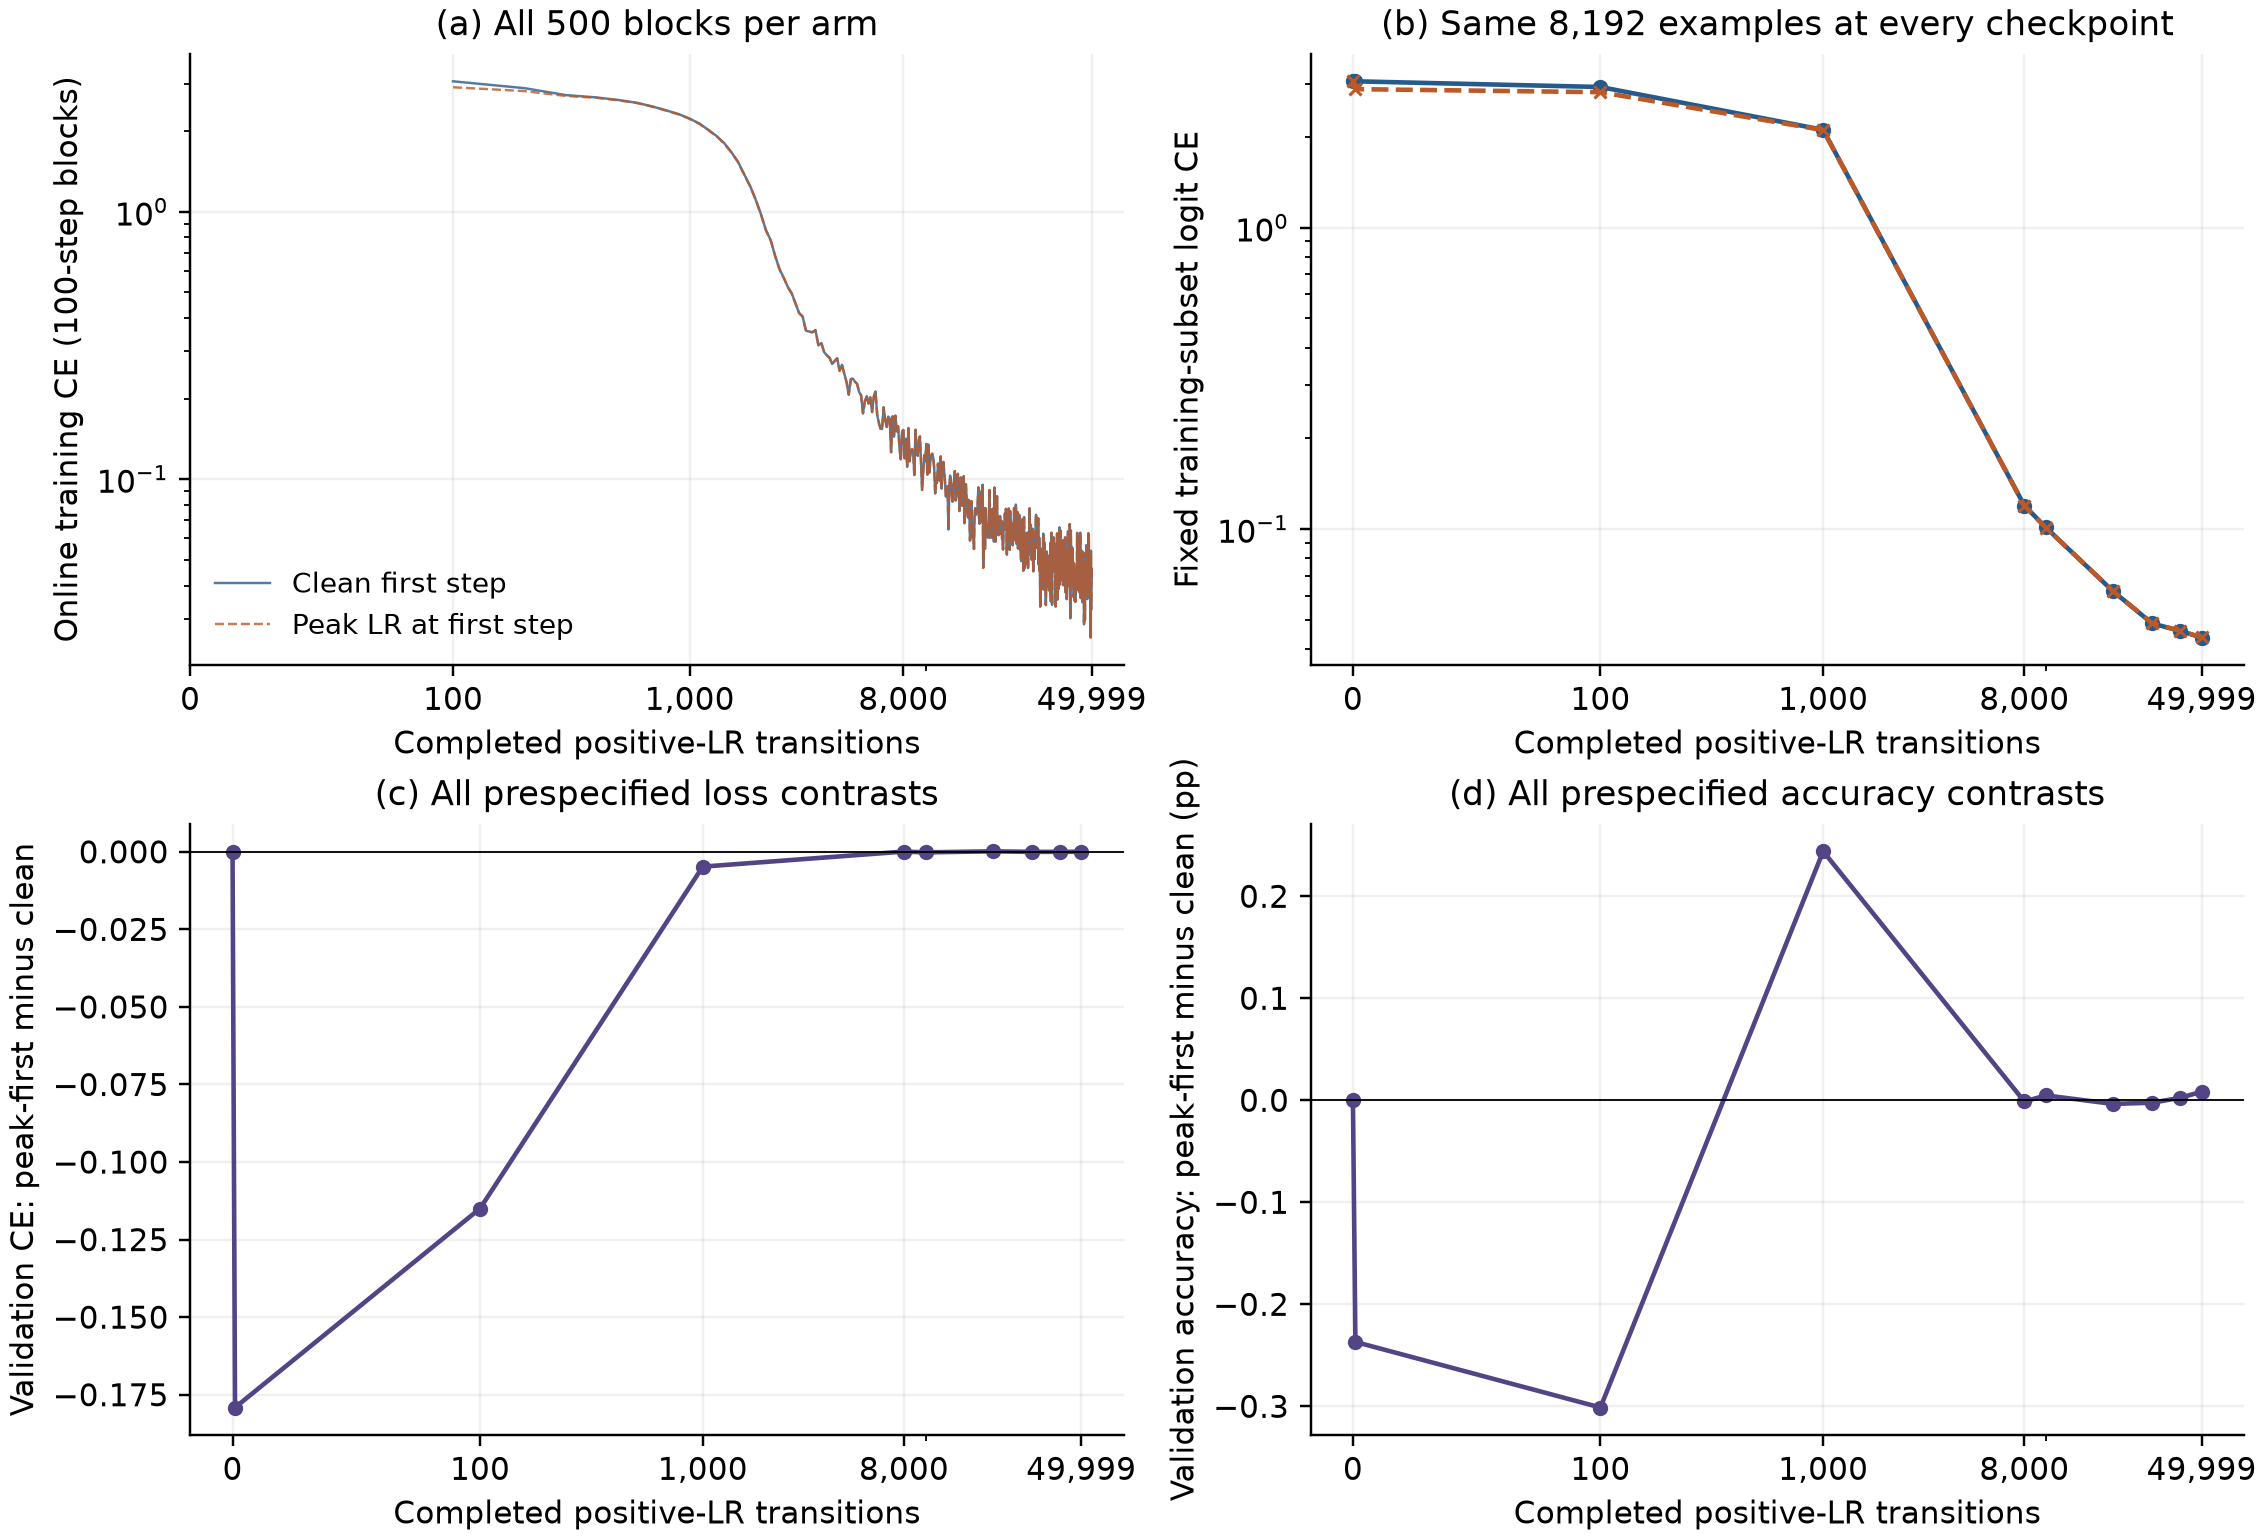
\includegraphics[width=0.98\linewidth,height=\textheight,keepaspectratio,height=0.72\textheight,keepaspectratio]{../figures/figS9_peak_first_training_and_differences.png}
\caption{All online training CE blocks, fixed training-subset checkpoint loss and prespecified validation contrasts. Online losses come from changing model states and dropout; checkpoint subset losses use evaluation mode. The two statistics are distinct. Differences are peak-first minus clean.}
\end{figure}

Every 100-transition online-loss block and the final 99-transition block is included in the machine-readable online-training table: 500 blocks per arm, 1,000 total. The complete 42 checkpoint/population/arm records are verified from raw logits and labels; the raw-logit verification table gives saved and independently recomputed CE and accuracy. Stable log-sum-exp is applied directly to uncapped logits and averaged over examples. Maximum absolute CE disagreement is 7.99e-15; all accuracies agree exactly. Example identities and labels agree across both arms and all checkpoints in each population.

\Needspace{16\baselineskip}

\section{Table S20 Per-arm budget and measured cost}\label{table-s20-per-arm-budget-and-measured-cost}

\begin{longtable}[]{@{}
  >{\raggedright\arraybackslash}p{(\linewidth - 10\tabcolsep) * \real{0.1667}}
  >{\raggedleft\arraybackslash}p{(\linewidth - 10\tabcolsep) * \real{0.1667}}
  >{\raggedleft\arraybackslash}p{(\linewidth - 10\tabcolsep) * \real{0.1667}}
  >{\raggedleft\arraybackslash}p{(\linewidth - 10\tabcolsep) * \real{0.1667}}
  >{\raggedleft\arraybackslash}p{(\linewidth - 10\tabcolsep) * \real{0.1667}}
  >{\raggedleft\arraybackslash}p{(\linewidth - 10\tabcolsep) * \real{0.1667}}@{}}
\toprule\noalign{}
\begin{minipage}[b]{\linewidth}\raggedright
Arm
\end{minipage} & \begin{minipage}[b]{\linewidth}\raggedleft
Positive-LR steps
\end{minipage} & \begin{minipage}[b]{\linewidth}\raggedleft
Zero-LR steps
\end{minipage} & \begin{minipage}[b]{\linewidth}\raggedleft
Examples
\end{minipage} & \begin{minipage}[b]{\linewidth}\raggedleft
Instrumented training (min)
\end{minipage} & \begin{minipage}[b]{\linewidth}\raggedleft
Evaluation (min)
\end{minipage} \\
\midrule\noalign{}
\endhead
\bottomrule\noalign{}
\endlastfoot
clean & 49,999 & 0 & 1,599,968 & 34.795 & 4.966 \\
peak-first & 49,999 & 0 & 1,599,968 & 34.955 & 4.927 \\
\end{longtable}

Shared recorded data-loading time is 83.685 seconds and checkpoint time 31.106 seconds. The closed training session totals 4,969.857 seconds (82.831 minutes); these component clocks do not account for every logging/control operation and must not be added to the total again. Training includes finite-state checks and the specified displacement instrumentation. GPU process peaks during the two arm intervals are 513,183,744 and 531,718,656 allocated bytes; both models remain resident. The maximum reported reserved memory is 601,882,624 bytes. These are not independent per-model memory footprints or an uninstrumented overhead comparison.

\section{Retained state and execution checks for the new pair}\label{retained-state-and-execution-checks-for-the-new-pair}

The three returned bundles contain 49 record/source files, 42 prediction files and five paired checkpoint files, with identical cross-bundle file manifests. Every member size and SHA-256 digest was checked. The audit reconstructs all 49,999 sampled batches from the saved sampler contract and checks 99,998 consumed-LR values, all 42 evaluation events and all 1,000 online-loss blocks. Each arm's rates match the prescribed schedule; rates after transition one match each other exactly. Independent cross-platform cosine evaluation differs only in the final floating-point bits, so the schedule audit uses relative tolerance 1e-12 and zero absolute tolerance. No failure, resumed segment, truncated record or zero-LR transition is recorded.

Full paired states are retained at 0, 1, 8,000 and 49,999, with a latest copy. Restricted tensor loading verifies finite parameters and Adam moments, all 55 active parameter-state counters, the prescribed groups/rates, paired RNG identity, sampler permutation/cursor/generator state and stored histories. The final retained state and latest state have identical scientific contents. The two first displacements recomputed from saved tensors match the trace. First-step optimizer moments are identical before later gradients diverge. These state checks are independent of the reported final accuracy.

The execution environment is Python 3.13.16, PyTorch 2.11.0+cu130, NumPy 2.1.3, datasets 4.8.5, huggingface-hub 1.33.0 and pyarrow 23.0.1 on one Tesla T4. A short serialization/resume probe with the actual model, loader and device matched uninterrupted execution exactly. The new research run itself completed in one uninterrupted segment. This evidence concerns the new paired runner; it does not retroactively certify the historical execution host, rollback path or cross-device reproducibility.

The primary final validation CE difference is +4.6952637067e-6. Official test CE is 0.057490380 versus 0.057494741, with accuracy 98.5986\% versus 98.6029\%. There is no prespecified equivalence margin or between-seed interval for this single pair. Its early lower CE and temporarily lower accuracy do not establish a damage-and-recovery mechanism. The tiny fixed-final contrast limits extrapolation from the LR=1.0 stress result without invalidating the historical observations.

\begin{figure}[htbp]
\centering
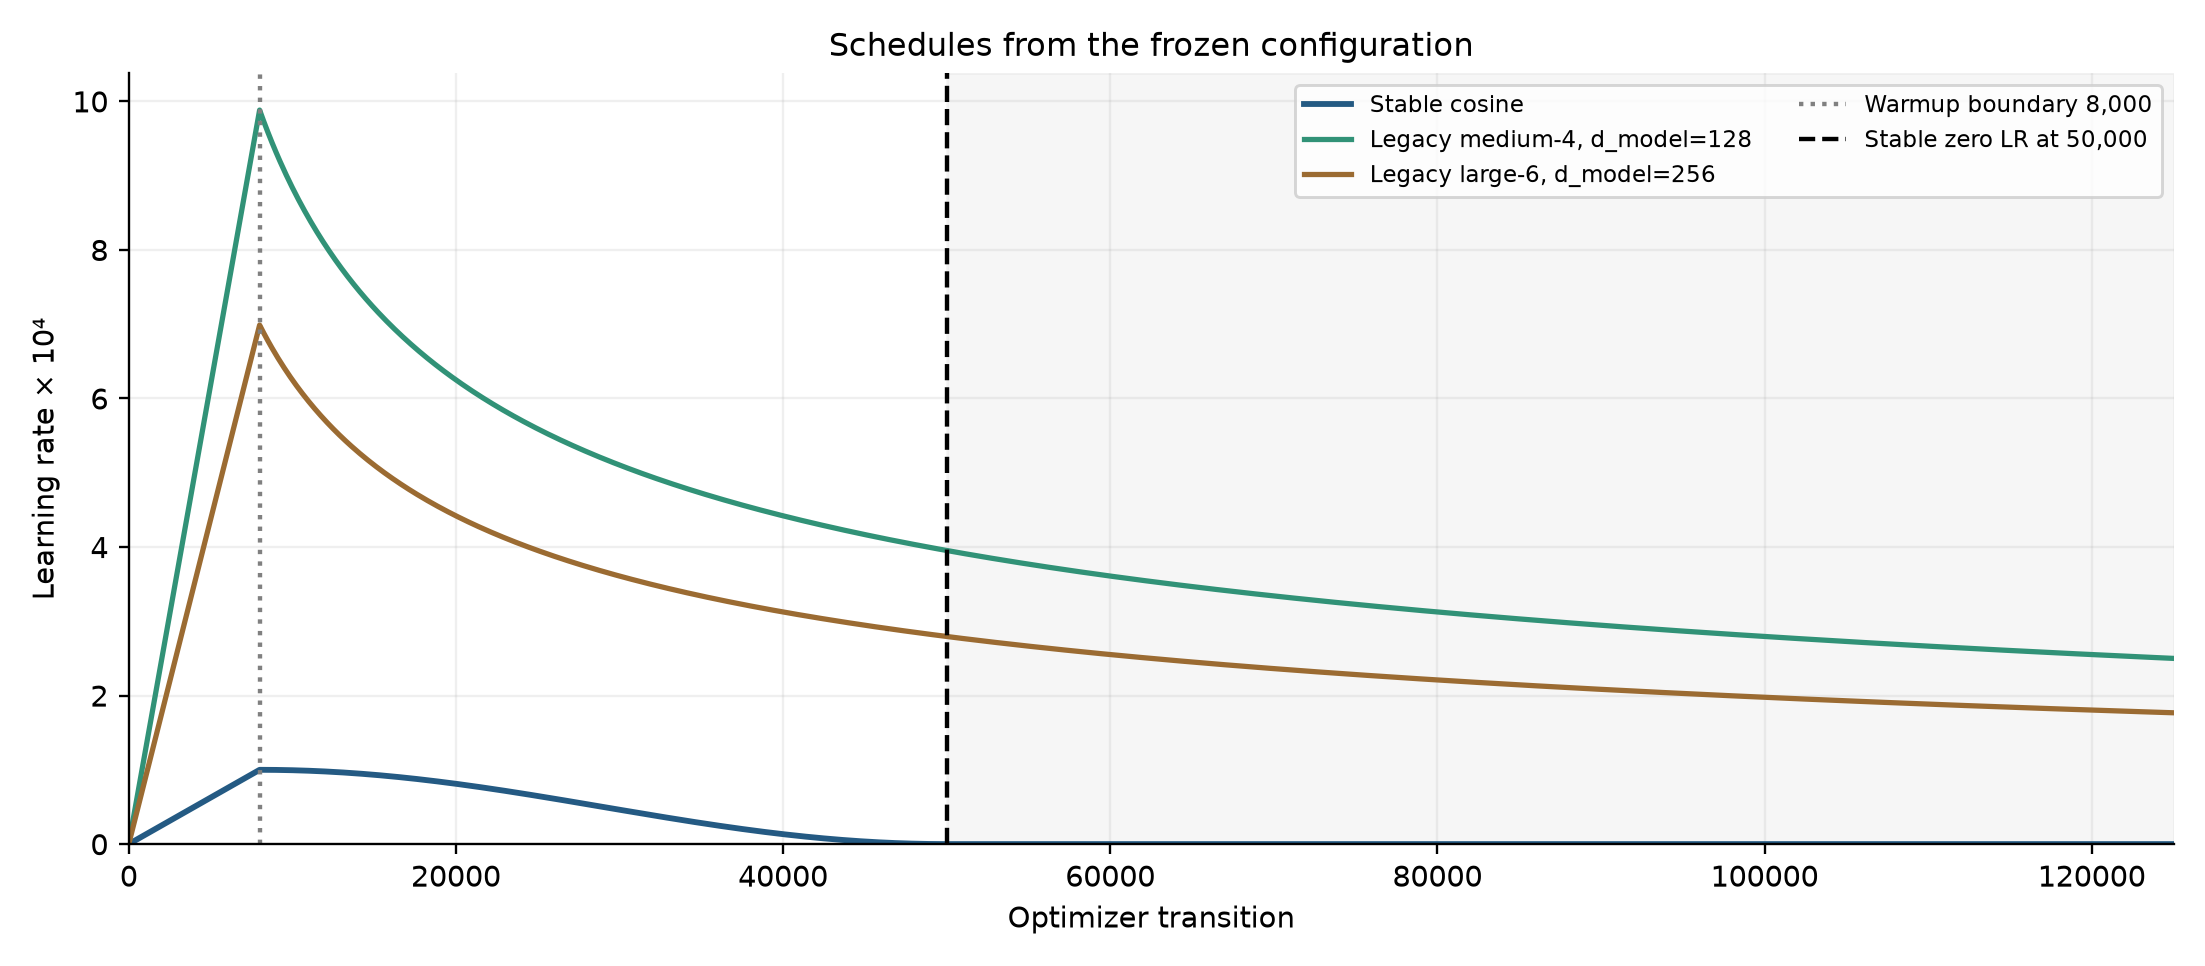
\includegraphics[width=0.98\linewidth,height=\textheight,keepaspectratio,height=0.72\textheight,keepaspectratio]{../figures/fig2_actual_configuration_schedule.png}
\caption{Stable and legacy schedules from the preserved configuration: widths 128/256, warmup 8,000 and stable zero boundary 50,000. Historical warmup 4,000 belongs to a separate cohort.}
\end{figure}

\begin{figure}[htbp]
\centering
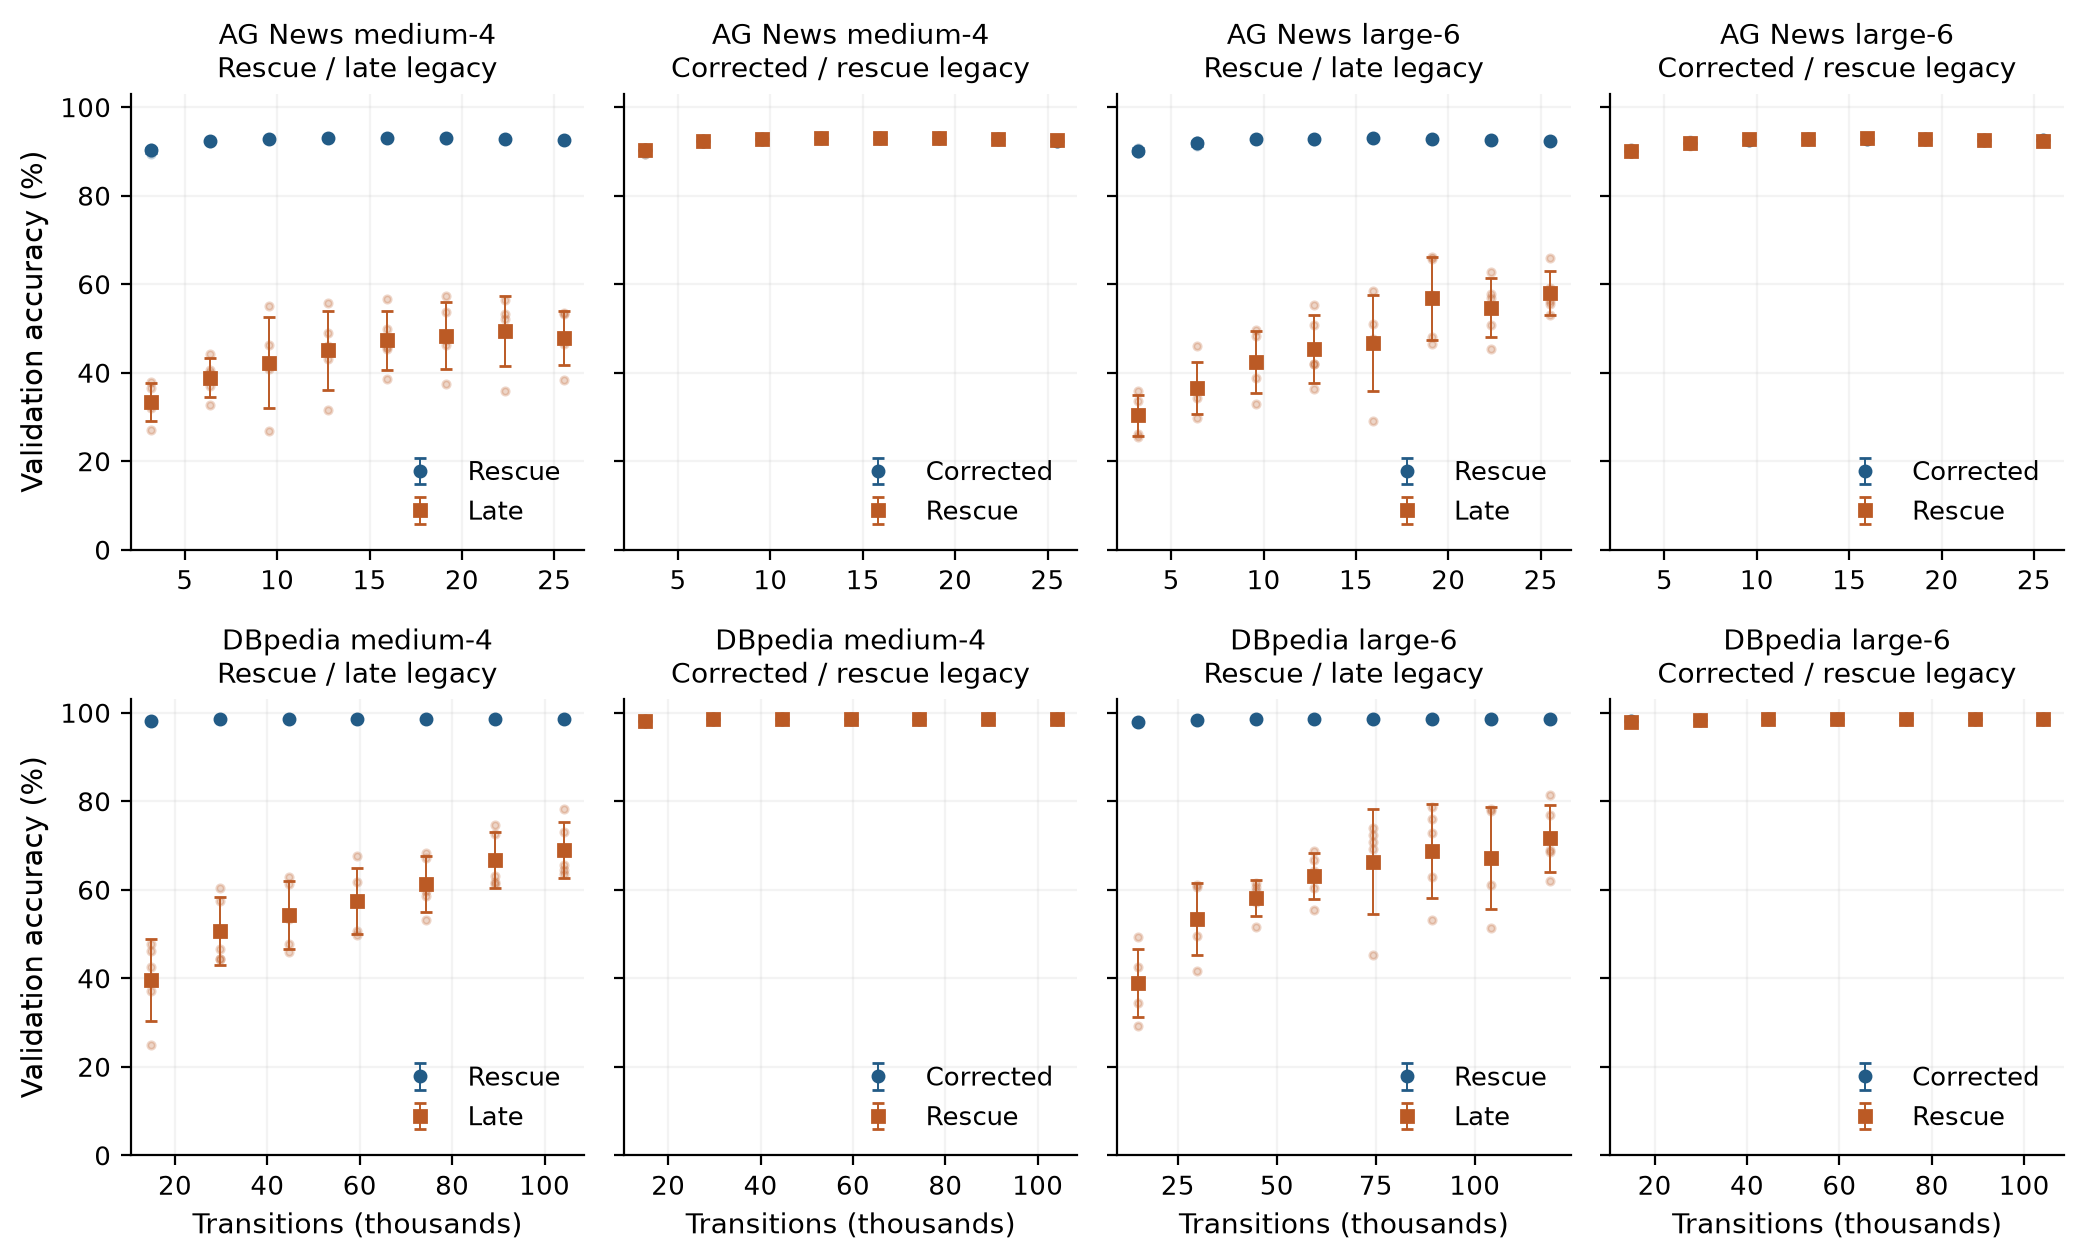
\includegraphics[width=0.98\linewidth,height=\textheight,keepaspectratio,height=0.72\textheight,keepaspectratio]{../figures/fig5_shared_step_legacy_validation.png}
\caption{Complete legacy validation comparisons at every common logged step within each contrast and all five seeds. Markers and bars show mean and sample SD. Stopping budgets differ; no interpolation or stopped-run carry-forward is used.}
\end{figure}

\section{Same-metric selected-checkpoint validation comparison}\label{same-metric-selected-checkpoint-validation-comparison}

DBpedia medium-4 rescue versus late execution: both retain later scheduler lag. Accuracy below is validation accuracy at the historically selected minimum-validation-loss epoch, not a newly selected accuracy maximum. The shared-step mean gap is 44.292857 percentage points at step 44,625; the selected-checkpoint mean gap is 5.822619 points. Unequal selected steps prevent interpreting the endpoint comparison as matched-compute recovery. Exact records and source paths are in \path{selected_validation_endpoint_pairs.csv}.

\begin{longtable}[]{@{}
  >{\raggedleft\arraybackslash}p{(\linewidth - 10\tabcolsep) * \real{0.1667}}
  >{\raggedleft\arraybackslash}p{(\linewidth - 10\tabcolsep) * \real{0.1667}}
  >{\raggedleft\arraybackslash}p{(\linewidth - 10\tabcolsep) * \real{0.1667}}
  >{\raggedleft\arraybackslash}p{(\linewidth - 10\tabcolsep) * \real{0.1667}}
  >{\raggedleft\arraybackslash}p{(\linewidth - 10\tabcolsep) * \real{0.1667}}
  >{\raggedleft\arraybackslash}p{(\linewidth - 10\tabcolsep) * \real{0.1667}}@{}}
\toprule\noalign{}
\begin{minipage}[b]{\linewidth}\raggedleft
Seed
\end{minipage} & \begin{minipage}[b]{\linewidth}\raggedleft
Late selected epoch
\end{minipage} & \begin{minipage}[b]{\linewidth}\raggedleft
Rescue selected epoch
\end{minipage} & \begin{minipage}[b]{\linewidth}\raggedleft
Late validation (\%)
\end{minipage} & \begin{minipage}[b]{\linewidth}\raggedleft
Rescue validation (\%)
\end{minipage} & \begin{minipage}[b]{\linewidth}\raggedleft
Difference (pp)
\end{minipage} \\
\midrule\noalign{}
\endhead
\bottomrule\noalign{}
\endlastfoot
42 & 30 & 2 & 94.388095 & 98.514286 & 4.126190 \\
123 & 28 & 6 & 93.766667 & 98.630952 & 4.864286 \\
456 & 30 & 3 & 92.364286 & 98.597619 & 6.233333 \\
789 & 29 & 4 & 92.559524 & 98.652381 & 6.092857 \\
2026 & 30 & 5 & 90.794048 & 98.590476 & 7.796429 \\
\end{longtable}

\section{Pretrained first rates and warmup lengths}\label{pretrained-first-rates-and-warmup-lengths}

The following values are identical across all five seeds within each task. The mismatch first rate is the configured peak; the safe first rate is peak divided by warmup length. All 20 safe/fault pairs are checked directly against archived manifests and first-transition traces in \path{pretrained_first_rates_and_warmup.csv}.

\begin{longtable}[]{@{}
  >{\raggedright\arraybackslash}p{(\linewidth - 8\tabcolsep) * \real{0.2000}}
  >{\raggedleft\arraybackslash}p{(\linewidth - 8\tabcolsep) * \real{0.2000}}
  >{\raggedleft\arraybackslash}p{(\linewidth - 8\tabcolsep) * \real{0.2000}}
  >{\raggedleft\arraybackslash}p{(\linewidth - 8\tabcolsep) * \real{0.2000}}
  >{\raggedleft\arraybackslash}p{(\linewidth - 8\tabcolsep) * \real{0.2000}}@{}}
\toprule\noalign{}
\begin{minipage}[b]{\linewidth}\raggedright
Task
\end{minipage} & \begin{minipage}[b]{\linewidth}\raggedleft
Total planned updates
\end{minipage} & \begin{minipage}[b]{\linewidth}\raggedleft
Warmup updates
\end{minipage} & \begin{minipage}[b]{\linewidth}\raggedleft
Fault first LR / peak
\end{minipage} & \begin{minipage}[b]{\linewidth}\raggedleft
Safe first LR
\end{minipage} \\
\midrule\noalign{}
\endhead
\bottomrule\noalign{}
\endlastfoot
ag\_news & 9564 & 957 & 2e-05 & 2.08986416e-08 \\
cifar10 & 4221 & 423 & 5e-05 & 1.1820331e-07 \\
dbpedia\_14 & 44625 & 4463 & 2e-05 & 4.48129061e-09 \\
wnut\_17 & 639 & 64 & 2e-05 & 3.125e-07 \\
\end{longtable}

The safe WNUT-17 trace reaches the peak at step 64 in every seed, inside the 1-100 calibration window. This may explain why its first-step fault does not exceed the primary displacement threshold, but no causal ablation tests that explanation. All five WNUT misses and the primary 35/40 count remain unchanged. Architecture and pretraining alone do not explain these records.

\end{document}
